\chapter{\textbf{Численные методы}}\label{ch:programming}
\section{\textbf{Задействованные математические библиотеки и пакеты}}\label{sec:programming/libraries}
Созданный в рамках данной работы программный комплекс реализован на двух языках. Ресурсоёмкие части реализованы на C++ и компилируются
в виде динамических библиотек, которые затем подключаются в код на Python с помощью библиотеки ctypes\cite{ctypes}. В коде на
Python реализована первичная обработка начальных данных, сведение воедино результатов вычислений и, наконец, вывод.

Одной из базовых задач при исполнении данной работы был подбор и освоение программных математических библиотек и
пакетов. Как уже отмечалось во введение, требованием к работе было использование свободного программного обеспечения,
тогда выбор становится очевиден.

В коде на Python это пакет NumPy\cite{harris2020array} и SciPy\cite{2020SciPy-NMeth}. Оба
написаны на С, С++ и Fortran и позволяют значительно ускорить вычисления, не теряя при этом в удобстве программирования
на Python. Numpy вводит особый тип данных, схожий с массивами, но поддерживающий исполнение различных математических операций.
Основное приложение NumPy "---программная реализация матриц, кроме того, с его помощью можно избежать чрезмерное употребление
циклов в коде, которые, сами по себе, в Python достаточно медленные. Функционал в SciPy достаточно обширен и включает в
себя алгоритмы численного интегрирования и дифференцирования, интерполяции, решения дифференциальных и систем линейных
уравнений, вычисления специальных функций. Оба пакета выпускаются под модифицированной лицензией
BSD\cite{numpy-license}\cite{scipy-license}, допускающей их свободное неограниченное использование, в том числе
встраивание в собственные проприетарные программы.

В коде на C++ это библиотека GNU Scientific Library\cite{galassi2018scientific}. Она написана на C совместимым с C++
образом, реализует работу с комплексными числами (впрочем, на практике удобней использовать те комплексные числа,
которые предоставляет сам С++) и разнообразные математические алгоритмы "---в основном всё то же, что уже перечислялось
выше для SciPy. GNU Scientific Library выпускается под лицензией GNU GPL третьей версии\cite{gsl-license} "---она
также допускает свободное использование, но создаёт требования при распространении программ, использующих данную
библиотеку, а именно, они также должны быть лицензированы под GNU GPL (либо под некоторыми другими совместимыми
лицензиями).

\section{\textbf{Геометрические векторы}}\label{sec:programming/vectors}
Для реализации формул, входящих в состав методов присоединённых плоских волн и рассеяных волн, было необходимо
реализовать работу с геометрическими векторами, записанными как в декартовых, так и сферических координатах, а также
их перевод из одной системы координат в другую. Соответствующий код на C++ был реализован в виде двух отдельных
классов: \texttt{coords\_cartesian} и \texttt{coords\_spherical}, как видно из названия, один позволяет записывать вектора
в декартовых координатах, а другой "---в сферических. С помощью функционала перегрузки операторов, предоставляемого C++,
реализовано сложение и вычитание представленных таким образом векторов, отдельные методы позволяют вычислять норму,
производить декартовое перемножение векторов, вычислять угол между векторами и переводить их из одной системы координат
в другую. Соответствующий код представлен в приложении~\cref{app:coordscpp}.

В той части кода, что написана на Python, соответствующий функционал реализован в виде единого класса \texttt{Vector},
который сразу хранит информацию как о декартовых координатах, так и о сферических "---см. приложение~\cref{app:vectorpy}.

\section{\textbf{Интегралы Гаунта}}\label{sec:programming/gaunt}
Интегралы Гаунта расчитываются по определению по формуле~\eqref{eq:gaunt}. Для этого с помощью средств SciPy
высчитывается сферическая функция\cite{scipy-spherical}, а затем она переводится в вещественную форму\cite{whittaker2014course}.
Далее следует численное интегрирование\cite{scipy-dblquad}, в результате которого получаем трёхмерную матрицу, индексами
которой являются упорядоченные пары $(l, m)$. Это матрица затем сохраняется в бинарный файл\cite{numpy-save} и может быть
сразу использована в дальнейшем без необходимости делать повторные расчёты.

\section{\textbf{Решение радиального уравнения}}\label{sec:programming/numerov}
Радиальное уравнение \eqref{eq:radialEquation} заменой
\begin{equation}\label{eq:radialFunctionChange}
  R_l(E, r) = \frac{P_{l E}(r)}{r}
\end{equation}

приводится к виду
\begin{equation}
  P_{l E}''(r)
  - \left(\frac{l \left(l + 1 \right)}{r^2} + V(r) - E\right) P_{l E}(r) = 0.
\end{equation}

Последнее может быть решено с помощью метода Нумерова. Полное описание метода можно найти в
книге~\cite{numerov}, остановимся лишь на его практической реализации.

Решение ДУ находится в виде последовательности точек. Из физических соображений, $P_{l E}(0) = 0$. Таким образом,
сразу известна первая точка решения. Вторая точка может быть задана произвольно, при этом $P_{l E}(r)$
будет найдена с точностью до постоянного множителя, который впоследствии вычисляется из условия нормировки. Если
заданы две точки, любые последующие могут быть высчитаны\cite{numerov-short} с помощью формулы
\begin{equation}
  P_{n} = \frac{(12-10f_{n-1}) P_{n-1}-f_{n-2}P_{n-2}}{f_{n}},
\end{equation}

где
\begin{equation}
f_n \equiv \left( 1 + \frac{h^2}{12}\left({\frac{l \left(l + 1 \right)}{r^2} + V(r) - E} \right) \right),
\end{equation}

а h "---шаг по аргументу функции.

Программный код, реализующий метод Нумерова, приведен в приложении~\cref{app:numerovcpp}. Для быстродействия код
написан на C++
и компилируется как динамическая библиотека, которая впоследствии может быть использована в программе на Python с
помощью библиотеки ctypes\cite{ctypes}.

Алгоритм можно упрощённо описать несколькими этапами:
\begin{enumerate}
    \item Построение интерполирующей функции для потенциала, переданного из программы на Python в виде
    последовательности точек.
    \item Решение ДУ для заданного потенциала, энергии и орбитального квантового числа методом Нумерова с малым шагом h
    "---при этом получается функция $P_{l E}(r)$, представленная большим числом точек.
    \item Построение интерполирующей функции для $P_{l E}(r)$.
    \item Интегрирование полученной интерполирующей функции, расчёт нормировочного коэффициента.
    \item Расчёт функции $R(E, r)$ как последовательности точек, согласно~\eqref{eq:radialFunctionChange}. При этом в
    первой точке получается неопределённость вида $\frac{0}{0}$, которая будет раскрыта в дальнейшем. Число точек,
    для экономии памяти и ускорения построения графиков, делается меньшим, чем изначально посчитанное "---в количестве,
    заданном программой на Python.
    \item Построение производной радиальной функции численными методами\cite{Fornberg1988GenerationOF} начиная с первой
    точки.
    \item Вычисление второй производной радиальной функции во второй точке.
    \item В допущении, что вторую производную радиальной функции при малых значениях аргумента можно считать постоянной,
    вычисление первой производной радиальной функции в нуле по формуле
    \begin{equation}
      R'_0 = R'_1 - R''_1 \tilde{h},
    \end{equation}

    где $\tilde{h}$ "---шаг по аргументу $R(E, r)$.

    \item Вычисление радиальной функции в нуле по формуле
    \begin{equation}
      R_0 = R_1 - R'_0 \tilde{h}.
    \end{equation}
\end{enumerate}

На рисунке~\cref{fig:radial-functions} приведены расчитанные таким образом радиальные функции на примере атома водорода
в различных состояниях. Потенциал при этом задаётся аналитически как
\begin{equation}
V(r) = -\frac{2}{r}.
\end{equation}

\begin{figure}[ht]
    \centerfloat{
        \ifdefmacro{\tikzsetnextfilename}{\tikzsetnextfilename{tikz_example_compiled}}{}% присваиваемое предкомпилированному pdf имя файла (не обязательно)
        %% Creator: Matplotlib, PGF backend
%%
%% To include the figure in your LaTeX document, write
%%   \input{<filename>.pgf}
%%
%% Make sure the required packages are loaded in your preamble
%%   \usepackage{pgf}
%%
%% and, on pdftex
%%   \usepackage[utf8]{inputenc}\DeclareUnicodeCharacter{2212}{-}
%%
%% or, on luatex and xetex
%%   \usepackage{unicode-math}
%%
%% Figures using additional raster images can only be included by \input if
%% they are in the same directory as the main LaTeX file. For loading figures
%% from other directories you can use the `import` package
%%   \usepackage{import}
%%
%% and then include the figures with
%%   \import{<path to file>}{<filename>.pgf}
%%
%% Matplotlib used the following preamble
%%   \usepackage{fontspec}
%%   \setmainfont{DejaVuSerif.ttf}[Path=/home/yernende/.local/lib/python3.8/site-packages/matplotlib/mpl-data/fonts/ttf/]
%%   \setsansfont{DejaVuSans.ttf}[Path=/home/yernende/.local/lib/python3.8/site-packages/matplotlib/mpl-data/fonts/ttf/]
%%   \setmonofont{DejaVuSansMono.ttf}[Path=/home/yernende/.local/lib/python3.8/site-packages/matplotlib/mpl-data/fonts/ttf/]
%%
\begingroup%
\makeatletter%
\begin{pgfpicture}%
\pgfpathrectangle{\pgfpointorigin}{\pgfqpoint{6.400000in}{4.800000in}}%
\pgfusepath{use as bounding box, clip}%
\begin{pgfscope}%
\pgfsetbuttcap%
\pgfsetmiterjoin%
\definecolor{currentfill}{rgb}{1.000000,1.000000,1.000000}%
\pgfsetfillcolor{currentfill}%
\pgfsetlinewidth{0.000000pt}%
\definecolor{currentstroke}{rgb}{1.000000,1.000000,1.000000}%
\pgfsetstrokecolor{currentstroke}%
\pgfsetdash{}{0pt}%
\pgfpathmoveto{\pgfqpoint{0.000000in}{0.000000in}}%
\pgfpathlineto{\pgfqpoint{6.400000in}{0.000000in}}%
\pgfpathlineto{\pgfqpoint{6.400000in}{4.800000in}}%
\pgfpathlineto{\pgfqpoint{0.000000in}{4.800000in}}%
\pgfpathclose%
\pgfusepath{fill}%
\end{pgfscope}%
\begin{pgfscope}%
\pgfsetbuttcap%
\pgfsetmiterjoin%
\definecolor{currentfill}{rgb}{1.000000,1.000000,1.000000}%
\pgfsetfillcolor{currentfill}%
\pgfsetlinewidth{0.000000pt}%
\definecolor{currentstroke}{rgb}{0.000000,0.000000,0.000000}%
\pgfsetstrokecolor{currentstroke}%
\pgfsetstrokeopacity{0.000000}%
\pgfsetdash{}{0pt}%
\pgfpathmoveto{\pgfqpoint{0.554722in}{2.712222in}}%
\pgfpathlineto{\pgfqpoint{1.927143in}{2.712222in}}%
\pgfpathlineto{\pgfqpoint{1.927143in}{4.426667in}}%
\pgfpathlineto{\pgfqpoint{0.554722in}{4.426667in}}%
\pgfpathclose%
\pgfusepath{fill}%
\end{pgfscope}%
\begin{pgfscope}%
\pgfsetbuttcap%
\pgfsetroundjoin%
\definecolor{currentfill}{rgb}{0.000000,0.000000,0.000000}%
\pgfsetfillcolor{currentfill}%
\pgfsetlinewidth{0.803000pt}%
\definecolor{currentstroke}{rgb}{0.000000,0.000000,0.000000}%
\pgfsetstrokecolor{currentstroke}%
\pgfsetdash{}{0pt}%
\pgfsys@defobject{currentmarker}{\pgfqpoint{0.000000in}{-0.048611in}}{\pgfqpoint{0.000000in}{0.000000in}}{%
\pgfpathmoveto{\pgfqpoint{0.000000in}{0.000000in}}%
\pgfpathlineto{\pgfqpoint{0.000000in}{-0.048611in}}%
\pgfusepath{stroke,fill}%
}%
\begin{pgfscope}%
\pgfsys@transformshift{0.617105in}{2.712222in}%
\pgfsys@useobject{currentmarker}{}%
\end{pgfscope}%
\end{pgfscope}%
\begin{pgfscope}%
\definecolor{textcolor}{rgb}{0.000000,0.000000,0.000000}%
\pgfsetstrokecolor{textcolor}%
\pgfsetfillcolor{textcolor}%
\pgftext[x=0.617105in,y=2.615000in,,top]{\color{textcolor}\sffamily\fontsize{10.000000}{12.000000}\selectfont 0}%
\end{pgfscope}%
\begin{pgfscope}%
\pgfsetbuttcap%
\pgfsetroundjoin%
\definecolor{currentfill}{rgb}{0.000000,0.000000,0.000000}%
\pgfsetfillcolor{currentfill}%
\pgfsetlinewidth{0.803000pt}%
\definecolor{currentstroke}{rgb}{0.000000,0.000000,0.000000}%
\pgfsetstrokecolor{currentstroke}%
\pgfsetdash{}{0pt}%
\pgfsys@defobject{currentmarker}{\pgfqpoint{0.000000in}{-0.048611in}}{\pgfqpoint{0.000000in}{0.000000in}}{%
\pgfpathmoveto{\pgfqpoint{0.000000in}{0.000000in}}%
\pgfpathlineto{\pgfqpoint{0.000000in}{-0.048611in}}%
\pgfusepath{stroke,fill}%
}%
\begin{pgfscope}%
\pgfsys@transformshift{1.240933in}{2.712222in}%
\pgfsys@useobject{currentmarker}{}%
\end{pgfscope}%
\end{pgfscope}%
\begin{pgfscope}%
\definecolor{textcolor}{rgb}{0.000000,0.000000,0.000000}%
\pgfsetstrokecolor{textcolor}%
\pgfsetfillcolor{textcolor}%
\pgftext[x=1.240933in,y=2.615000in,,top]{\color{textcolor}\sffamily\fontsize{10.000000}{12.000000}\selectfont 5}%
\end{pgfscope}%
\begin{pgfscope}%
\pgfsetbuttcap%
\pgfsetroundjoin%
\definecolor{currentfill}{rgb}{0.000000,0.000000,0.000000}%
\pgfsetfillcolor{currentfill}%
\pgfsetlinewidth{0.803000pt}%
\definecolor{currentstroke}{rgb}{0.000000,0.000000,0.000000}%
\pgfsetstrokecolor{currentstroke}%
\pgfsetdash{}{0pt}%
\pgfsys@defobject{currentmarker}{\pgfqpoint{0.000000in}{-0.048611in}}{\pgfqpoint{0.000000in}{0.000000in}}{%
\pgfpathmoveto{\pgfqpoint{0.000000in}{0.000000in}}%
\pgfpathlineto{\pgfqpoint{0.000000in}{-0.048611in}}%
\pgfusepath{stroke,fill}%
}%
\begin{pgfscope}%
\pgfsys@transformshift{1.864761in}{2.712222in}%
\pgfsys@useobject{currentmarker}{}%
\end{pgfscope}%
\end{pgfscope}%
\begin{pgfscope}%
\definecolor{textcolor}{rgb}{0.000000,0.000000,0.000000}%
\pgfsetstrokecolor{textcolor}%
\pgfsetfillcolor{textcolor}%
\pgftext[x=1.864761in,y=2.615000in,,top]{\color{textcolor}\sffamily\fontsize{10.000000}{12.000000}\selectfont 10}%
\end{pgfscope}%
\begin{pgfscope}%
\pgfsetbuttcap%
\pgfsetroundjoin%
\definecolor{currentfill}{rgb}{0.000000,0.000000,0.000000}%
\pgfsetfillcolor{currentfill}%
\pgfsetlinewidth{0.803000pt}%
\definecolor{currentstroke}{rgb}{0.000000,0.000000,0.000000}%
\pgfsetstrokecolor{currentstroke}%
\pgfsetdash{}{0pt}%
\pgfsys@defobject{currentmarker}{\pgfqpoint{-0.048611in}{0.000000in}}{\pgfqpoint{-0.000000in}{0.000000in}}{%
\pgfpathmoveto{\pgfqpoint{-0.000000in}{0.000000in}}%
\pgfpathlineto{\pgfqpoint{-0.048611in}{0.000000in}}%
\pgfusepath{stroke,fill}%
}%
\begin{pgfscope}%
\pgfsys@transformshift{0.554722in}{2.790095in}%
\pgfsys@useobject{currentmarker}{}%
\end{pgfscope}%
\end{pgfscope}%
\begin{pgfscope}%
\definecolor{textcolor}{rgb}{0.000000,0.000000,0.000000}%
\pgfsetstrokecolor{textcolor}%
\pgfsetfillcolor{textcolor}%
\pgftext[x=0.236621in, y=2.737333in, left, base]{\color{textcolor}\sffamily\fontsize{10.000000}{12.000000}\selectfont 0.0}%
\end{pgfscope}%
\begin{pgfscope}%
\pgfsetbuttcap%
\pgfsetroundjoin%
\definecolor{currentfill}{rgb}{0.000000,0.000000,0.000000}%
\pgfsetfillcolor{currentfill}%
\pgfsetlinewidth{0.803000pt}%
\definecolor{currentstroke}{rgb}{0.000000,0.000000,0.000000}%
\pgfsetstrokecolor{currentstroke}%
\pgfsetdash{}{0pt}%
\pgfsys@defobject{currentmarker}{\pgfqpoint{-0.048611in}{0.000000in}}{\pgfqpoint{-0.000000in}{0.000000in}}{%
\pgfpathmoveto{\pgfqpoint{-0.000000in}{0.000000in}}%
\pgfpathlineto{\pgfqpoint{-0.048611in}{0.000000in}}%
\pgfusepath{stroke,fill}%
}%
\begin{pgfscope}%
\pgfsys@transformshift{0.554722in}{3.179785in}%
\pgfsys@useobject{currentmarker}{}%
\end{pgfscope}%
\end{pgfscope}%
\begin{pgfscope}%
\definecolor{textcolor}{rgb}{0.000000,0.000000,0.000000}%
\pgfsetstrokecolor{textcolor}%
\pgfsetfillcolor{textcolor}%
\pgftext[x=0.236621in, y=3.127024in, left, base]{\color{textcolor}\sffamily\fontsize{10.000000}{12.000000}\selectfont 0.5}%
\end{pgfscope}%
\begin{pgfscope}%
\pgfsetbuttcap%
\pgfsetroundjoin%
\definecolor{currentfill}{rgb}{0.000000,0.000000,0.000000}%
\pgfsetfillcolor{currentfill}%
\pgfsetlinewidth{0.803000pt}%
\definecolor{currentstroke}{rgb}{0.000000,0.000000,0.000000}%
\pgfsetstrokecolor{currentstroke}%
\pgfsetdash{}{0pt}%
\pgfsys@defobject{currentmarker}{\pgfqpoint{-0.048611in}{0.000000in}}{\pgfqpoint{-0.000000in}{0.000000in}}{%
\pgfpathmoveto{\pgfqpoint{-0.000000in}{0.000000in}}%
\pgfpathlineto{\pgfqpoint{-0.048611in}{0.000000in}}%
\pgfusepath{stroke,fill}%
}%
\begin{pgfscope}%
\pgfsys@transformshift{0.554722in}{3.569476in}%
\pgfsys@useobject{currentmarker}{}%
\end{pgfscope}%
\end{pgfscope}%
\begin{pgfscope}%
\definecolor{textcolor}{rgb}{0.000000,0.000000,0.000000}%
\pgfsetstrokecolor{textcolor}%
\pgfsetfillcolor{textcolor}%
\pgftext[x=0.236621in, y=3.516714in, left, base]{\color{textcolor}\sffamily\fontsize{10.000000}{12.000000}\selectfont 1.0}%
\end{pgfscope}%
\begin{pgfscope}%
\pgfsetbuttcap%
\pgfsetroundjoin%
\definecolor{currentfill}{rgb}{0.000000,0.000000,0.000000}%
\pgfsetfillcolor{currentfill}%
\pgfsetlinewidth{0.803000pt}%
\definecolor{currentstroke}{rgb}{0.000000,0.000000,0.000000}%
\pgfsetstrokecolor{currentstroke}%
\pgfsetdash{}{0pt}%
\pgfsys@defobject{currentmarker}{\pgfqpoint{-0.048611in}{0.000000in}}{\pgfqpoint{-0.000000in}{0.000000in}}{%
\pgfpathmoveto{\pgfqpoint{-0.000000in}{0.000000in}}%
\pgfpathlineto{\pgfqpoint{-0.048611in}{0.000000in}}%
\pgfusepath{stroke,fill}%
}%
\begin{pgfscope}%
\pgfsys@transformshift{0.554722in}{3.959166in}%
\pgfsys@useobject{currentmarker}{}%
\end{pgfscope}%
\end{pgfscope}%
\begin{pgfscope}%
\definecolor{textcolor}{rgb}{0.000000,0.000000,0.000000}%
\pgfsetstrokecolor{textcolor}%
\pgfsetfillcolor{textcolor}%
\pgftext[x=0.236621in, y=3.906404in, left, base]{\color{textcolor}\sffamily\fontsize{10.000000}{12.000000}\selectfont 1.5}%
\end{pgfscope}%
\begin{pgfscope}%
\pgfsetbuttcap%
\pgfsetroundjoin%
\definecolor{currentfill}{rgb}{0.000000,0.000000,0.000000}%
\pgfsetfillcolor{currentfill}%
\pgfsetlinewidth{0.803000pt}%
\definecolor{currentstroke}{rgb}{0.000000,0.000000,0.000000}%
\pgfsetstrokecolor{currentstroke}%
\pgfsetdash{}{0pt}%
\pgfsys@defobject{currentmarker}{\pgfqpoint{-0.048611in}{0.000000in}}{\pgfqpoint{-0.000000in}{0.000000in}}{%
\pgfpathmoveto{\pgfqpoint{-0.000000in}{0.000000in}}%
\pgfpathlineto{\pgfqpoint{-0.048611in}{0.000000in}}%
\pgfusepath{stroke,fill}%
}%
\begin{pgfscope}%
\pgfsys@transformshift{0.554722in}{4.348856in}%
\pgfsys@useobject{currentmarker}{}%
\end{pgfscope}%
\end{pgfscope}%
\begin{pgfscope}%
\definecolor{textcolor}{rgb}{0.000000,0.000000,0.000000}%
\pgfsetstrokecolor{textcolor}%
\pgfsetfillcolor{textcolor}%
\pgftext[x=0.236621in, y=4.296095in, left, base]{\color{textcolor}\sffamily\fontsize{10.000000}{12.000000}\selectfont 2.0}%
\end{pgfscope}%
\begin{pgfscope}%
\pgfpathrectangle{\pgfqpoint{0.554722in}{2.712222in}}{\pgfqpoint{1.372421in}{1.714444in}}%
\pgfusepath{clip}%
\pgfsetrectcap%
\pgfsetroundjoin%
\pgfsetlinewidth{1.505625pt}%
\definecolor{currentstroke}{rgb}{0.121569,0.466667,0.705882}%
\pgfsetstrokecolor{currentstroke}%
\pgfsetdash{}{0pt}%
\pgfpathmoveto{\pgfqpoint{0.617105in}{4.348737in}}%
\pgfpathlineto{\pgfqpoint{0.625590in}{4.246379in}}%
\pgfpathlineto{\pgfqpoint{0.642685in}{4.059913in}}%
\pgfpathlineto{\pgfqpoint{0.659779in}{3.897323in}}%
\pgfpathlineto{\pgfqpoint{0.676874in}{3.755551in}}%
\pgfpathlineto{\pgfqpoint{0.693968in}{3.631933in}}%
\pgfpathlineto{\pgfqpoint{0.711063in}{3.524142in}}%
\pgfpathlineto{\pgfqpoint{0.728157in}{3.430153in}}%
\pgfpathlineto{\pgfqpoint{0.745377in}{3.347641in}}%
\pgfpathlineto{\pgfqpoint{0.762596in}{3.275766in}}%
\pgfpathlineto{\pgfqpoint{0.779940in}{3.212734in}}%
\pgfpathlineto{\pgfqpoint{0.797285in}{3.157882in}}%
\pgfpathlineto{\pgfqpoint{0.814753in}{3.109829in}}%
\pgfpathlineto{\pgfqpoint{0.832472in}{3.067499in}}%
\pgfpathlineto{\pgfqpoint{0.850315in}{3.030533in}}%
\pgfpathlineto{\pgfqpoint{0.868408in}{2.998076in}}%
\pgfpathlineto{\pgfqpoint{0.886875in}{2.969461in}}%
\pgfpathlineto{\pgfqpoint{0.905717in}{2.944320in}}%
\pgfpathlineto{\pgfqpoint{0.925057in}{2.922174in}}%
\pgfpathlineto{\pgfqpoint{0.945146in}{2.902531in}}%
\pgfpathlineto{\pgfqpoint{0.966109in}{2.885141in}}%
\pgfpathlineto{\pgfqpoint{0.988070in}{2.869801in}}%
\pgfpathlineto{\pgfqpoint{1.011528in}{2.856139in}}%
\pgfpathlineto{\pgfqpoint{1.036734in}{2.844058in}}%
\pgfpathlineto{\pgfqpoint{1.064185in}{2.833401in}}%
\pgfpathlineto{\pgfqpoint{1.094506in}{2.824057in}}%
\pgfpathlineto{\pgfqpoint{1.128445in}{2.815969in}}%
\pgfpathlineto{\pgfqpoint{1.167376in}{2.809033in}}%
\pgfpathlineto{\pgfqpoint{1.213045in}{2.803228in}}%
\pgfpathlineto{\pgfqpoint{1.268322in}{2.798527in}}%
\pgfpathlineto{\pgfqpoint{1.338447in}{2.794901in}}%
\pgfpathlineto{\pgfqpoint{1.434152in}{2.792326in}}%
\pgfpathlineto{\pgfqpoint{1.583386in}{2.790767in}}%
\pgfpathlineto{\pgfqpoint{1.864761in}{2.790152in}}%
\pgfpathlineto{\pgfqpoint{1.864761in}{2.790152in}}%
\pgfusepath{stroke}%
\end{pgfscope}%
\begin{pgfscope}%
\pgfsetrectcap%
\pgfsetmiterjoin%
\pgfsetlinewidth{0.803000pt}%
\definecolor{currentstroke}{rgb}{0.000000,0.000000,0.000000}%
\pgfsetstrokecolor{currentstroke}%
\pgfsetdash{}{0pt}%
\pgfpathmoveto{\pgfqpoint{0.554722in}{2.712222in}}%
\pgfpathlineto{\pgfqpoint{0.554722in}{4.426667in}}%
\pgfusepath{stroke}%
\end{pgfscope}%
\begin{pgfscope}%
\pgfsetrectcap%
\pgfsetmiterjoin%
\pgfsetlinewidth{0.803000pt}%
\definecolor{currentstroke}{rgb}{0.000000,0.000000,0.000000}%
\pgfsetstrokecolor{currentstroke}%
\pgfsetdash{}{0pt}%
\pgfpathmoveto{\pgfqpoint{1.927143in}{2.712222in}}%
\pgfpathlineto{\pgfqpoint{1.927143in}{4.426667in}}%
\pgfusepath{stroke}%
\end{pgfscope}%
\begin{pgfscope}%
\pgfsetrectcap%
\pgfsetmiterjoin%
\pgfsetlinewidth{0.803000pt}%
\definecolor{currentstroke}{rgb}{0.000000,0.000000,0.000000}%
\pgfsetstrokecolor{currentstroke}%
\pgfsetdash{}{0pt}%
\pgfpathmoveto{\pgfqpoint{0.554722in}{2.712222in}}%
\pgfpathlineto{\pgfqpoint{1.927143in}{2.712222in}}%
\pgfusepath{stroke}%
\end{pgfscope}%
\begin{pgfscope}%
\pgfsetrectcap%
\pgfsetmiterjoin%
\pgfsetlinewidth{0.803000pt}%
\definecolor{currentstroke}{rgb}{0.000000,0.000000,0.000000}%
\pgfsetstrokecolor{currentstroke}%
\pgfsetdash{}{0pt}%
\pgfpathmoveto{\pgfqpoint{0.554722in}{4.426667in}}%
\pgfpathlineto{\pgfqpoint{1.927143in}{4.426667in}}%
\pgfusepath{stroke}%
\end{pgfscope}%
\begin{pgfscope}%
\definecolor{textcolor}{rgb}{0.000000,0.000000,0.000000}%
\pgfsetstrokecolor{textcolor}%
\pgfsetfillcolor{textcolor}%
\pgftext[x=1.240933in,y=4.510000in,,base]{\color{textcolor}\sffamily\fontsize{12.000000}{14.400000}\selectfont E = -1, l = 0}%
\end{pgfscope}%
\begin{pgfscope}%
\pgfsetbuttcap%
\pgfsetmiterjoin%
\definecolor{currentfill}{rgb}{1.000000,1.000000,1.000000}%
\pgfsetfillcolor{currentfill}%
\pgfsetlinewidth{0.000000pt}%
\definecolor{currentstroke}{rgb}{0.000000,0.000000,0.000000}%
\pgfsetstrokecolor{currentstroke}%
\pgfsetstrokeopacity{0.000000}%
\pgfsetdash{}{0pt}%
\pgfpathmoveto{\pgfqpoint{2.705556in}{2.712222in}}%
\pgfpathlineto{\pgfqpoint{4.077977in}{2.712222in}}%
\pgfpathlineto{\pgfqpoint{4.077977in}{4.426667in}}%
\pgfpathlineto{\pgfqpoint{2.705556in}{4.426667in}}%
\pgfpathclose%
\pgfusepath{fill}%
\end{pgfscope}%
\begin{pgfscope}%
\pgfsetbuttcap%
\pgfsetroundjoin%
\definecolor{currentfill}{rgb}{0.000000,0.000000,0.000000}%
\pgfsetfillcolor{currentfill}%
\pgfsetlinewidth{0.803000pt}%
\definecolor{currentstroke}{rgb}{0.000000,0.000000,0.000000}%
\pgfsetstrokecolor{currentstroke}%
\pgfsetdash{}{0pt}%
\pgfsys@defobject{currentmarker}{\pgfqpoint{0.000000in}{-0.048611in}}{\pgfqpoint{0.000000in}{0.000000in}}{%
\pgfpathmoveto{\pgfqpoint{0.000000in}{0.000000in}}%
\pgfpathlineto{\pgfqpoint{0.000000in}{-0.048611in}}%
\pgfusepath{stroke,fill}%
}%
\begin{pgfscope}%
\pgfsys@transformshift{2.767938in}{2.712222in}%
\pgfsys@useobject{currentmarker}{}%
\end{pgfscope}%
\end{pgfscope}%
\begin{pgfscope}%
\definecolor{textcolor}{rgb}{0.000000,0.000000,0.000000}%
\pgfsetstrokecolor{textcolor}%
\pgfsetfillcolor{textcolor}%
\pgftext[x=2.767938in,y=2.615000in,,top]{\color{textcolor}\sffamily\fontsize{10.000000}{12.000000}\selectfont 0}%
\end{pgfscope}%
\begin{pgfscope}%
\pgfsetbuttcap%
\pgfsetroundjoin%
\definecolor{currentfill}{rgb}{0.000000,0.000000,0.000000}%
\pgfsetfillcolor{currentfill}%
\pgfsetlinewidth{0.803000pt}%
\definecolor{currentstroke}{rgb}{0.000000,0.000000,0.000000}%
\pgfsetstrokecolor{currentstroke}%
\pgfsetdash{}{0pt}%
\pgfsys@defobject{currentmarker}{\pgfqpoint{0.000000in}{-0.048611in}}{\pgfqpoint{0.000000in}{0.000000in}}{%
\pgfpathmoveto{\pgfqpoint{0.000000in}{0.000000in}}%
\pgfpathlineto{\pgfqpoint{0.000000in}{-0.048611in}}%
\pgfusepath{stroke,fill}%
}%
\begin{pgfscope}%
\pgfsys@transformshift{3.391766in}{2.712222in}%
\pgfsys@useobject{currentmarker}{}%
\end{pgfscope}%
\end{pgfscope}%
\begin{pgfscope}%
\definecolor{textcolor}{rgb}{0.000000,0.000000,0.000000}%
\pgfsetstrokecolor{textcolor}%
\pgfsetfillcolor{textcolor}%
\pgftext[x=3.391766in,y=2.615000in,,top]{\color{textcolor}\sffamily\fontsize{10.000000}{12.000000}\selectfont 10}%
\end{pgfscope}%
\begin{pgfscope}%
\pgfsetbuttcap%
\pgfsetroundjoin%
\definecolor{currentfill}{rgb}{0.000000,0.000000,0.000000}%
\pgfsetfillcolor{currentfill}%
\pgfsetlinewidth{0.803000pt}%
\definecolor{currentstroke}{rgb}{0.000000,0.000000,0.000000}%
\pgfsetstrokecolor{currentstroke}%
\pgfsetdash{}{0pt}%
\pgfsys@defobject{currentmarker}{\pgfqpoint{0.000000in}{-0.048611in}}{\pgfqpoint{0.000000in}{0.000000in}}{%
\pgfpathmoveto{\pgfqpoint{0.000000in}{0.000000in}}%
\pgfpathlineto{\pgfqpoint{0.000000in}{-0.048611in}}%
\pgfusepath{stroke,fill}%
}%
\begin{pgfscope}%
\pgfsys@transformshift{4.015594in}{2.712222in}%
\pgfsys@useobject{currentmarker}{}%
\end{pgfscope}%
\end{pgfscope}%
\begin{pgfscope}%
\definecolor{textcolor}{rgb}{0.000000,0.000000,0.000000}%
\pgfsetstrokecolor{textcolor}%
\pgfsetfillcolor{textcolor}%
\pgftext[x=4.015594in,y=2.615000in,,top]{\color{textcolor}\sffamily\fontsize{10.000000}{12.000000}\selectfont 20}%
\end{pgfscope}%
\begin{pgfscope}%
\pgfsetbuttcap%
\pgfsetroundjoin%
\definecolor{currentfill}{rgb}{0.000000,0.000000,0.000000}%
\pgfsetfillcolor{currentfill}%
\pgfsetlinewidth{0.803000pt}%
\definecolor{currentstroke}{rgb}{0.000000,0.000000,0.000000}%
\pgfsetstrokecolor{currentstroke}%
\pgfsetdash{}{0pt}%
\pgfsys@defobject{currentmarker}{\pgfqpoint{-0.048611in}{0.000000in}}{\pgfqpoint{-0.000000in}{0.000000in}}{%
\pgfpathmoveto{\pgfqpoint{-0.000000in}{0.000000in}}%
\pgfpathlineto{\pgfqpoint{-0.048611in}{0.000000in}}%
\pgfusepath{stroke,fill}%
}%
\begin{pgfscope}%
\pgfsys@transformshift{2.705556in}{2.975963in}%
\pgfsys@useobject{currentmarker}{}%
\end{pgfscope}%
\end{pgfscope}%
\begin{pgfscope}%
\definecolor{textcolor}{rgb}{0.000000,0.000000,0.000000}%
\pgfsetstrokecolor{textcolor}%
\pgfsetfillcolor{textcolor}%
\pgftext[x=2.387454in, y=2.923202in, left, base]{\color{textcolor}\sffamily\fontsize{10.000000}{12.000000}\selectfont 0.0}%
\end{pgfscope}%
\begin{pgfscope}%
\pgfsetbuttcap%
\pgfsetroundjoin%
\definecolor{currentfill}{rgb}{0.000000,0.000000,0.000000}%
\pgfsetfillcolor{currentfill}%
\pgfsetlinewidth{0.803000pt}%
\definecolor{currentstroke}{rgb}{0.000000,0.000000,0.000000}%
\pgfsetstrokecolor{currentstroke}%
\pgfsetdash{}{0pt}%
\pgfsys@defobject{currentmarker}{\pgfqpoint{-0.048611in}{0.000000in}}{\pgfqpoint{-0.000000in}{0.000000in}}{%
\pgfpathmoveto{\pgfqpoint{-0.000000in}{0.000000in}}%
\pgfpathlineto{\pgfqpoint{-0.048611in}{0.000000in}}%
\pgfusepath{stroke,fill}%
}%
\begin{pgfscope}%
\pgfsys@transformshift{2.705556in}{3.364289in}%
\pgfsys@useobject{currentmarker}{}%
\end{pgfscope}%
\end{pgfscope}%
\begin{pgfscope}%
\definecolor{textcolor}{rgb}{0.000000,0.000000,0.000000}%
\pgfsetstrokecolor{textcolor}%
\pgfsetfillcolor{textcolor}%
\pgftext[x=2.387454in, y=3.311527in, left, base]{\color{textcolor}\sffamily\fontsize{10.000000}{12.000000}\selectfont 0.2}%
\end{pgfscope}%
\begin{pgfscope}%
\pgfsetbuttcap%
\pgfsetroundjoin%
\definecolor{currentfill}{rgb}{0.000000,0.000000,0.000000}%
\pgfsetfillcolor{currentfill}%
\pgfsetlinewidth{0.803000pt}%
\definecolor{currentstroke}{rgb}{0.000000,0.000000,0.000000}%
\pgfsetstrokecolor{currentstroke}%
\pgfsetdash{}{0pt}%
\pgfsys@defobject{currentmarker}{\pgfqpoint{-0.048611in}{0.000000in}}{\pgfqpoint{-0.000000in}{0.000000in}}{%
\pgfpathmoveto{\pgfqpoint{-0.000000in}{0.000000in}}%
\pgfpathlineto{\pgfqpoint{-0.048611in}{0.000000in}}%
\pgfusepath{stroke,fill}%
}%
\begin{pgfscope}%
\pgfsys@transformshift{2.705556in}{3.752615in}%
\pgfsys@useobject{currentmarker}{}%
\end{pgfscope}%
\end{pgfscope}%
\begin{pgfscope}%
\definecolor{textcolor}{rgb}{0.000000,0.000000,0.000000}%
\pgfsetstrokecolor{textcolor}%
\pgfsetfillcolor{textcolor}%
\pgftext[x=2.387454in, y=3.699853in, left, base]{\color{textcolor}\sffamily\fontsize{10.000000}{12.000000}\selectfont 0.4}%
\end{pgfscope}%
\begin{pgfscope}%
\pgfsetbuttcap%
\pgfsetroundjoin%
\definecolor{currentfill}{rgb}{0.000000,0.000000,0.000000}%
\pgfsetfillcolor{currentfill}%
\pgfsetlinewidth{0.803000pt}%
\definecolor{currentstroke}{rgb}{0.000000,0.000000,0.000000}%
\pgfsetstrokecolor{currentstroke}%
\pgfsetdash{}{0pt}%
\pgfsys@defobject{currentmarker}{\pgfqpoint{-0.048611in}{0.000000in}}{\pgfqpoint{-0.000000in}{0.000000in}}{%
\pgfpathmoveto{\pgfqpoint{-0.000000in}{0.000000in}}%
\pgfpathlineto{\pgfqpoint{-0.048611in}{0.000000in}}%
\pgfusepath{stroke,fill}%
}%
\begin{pgfscope}%
\pgfsys@transformshift{2.705556in}{4.140940in}%
\pgfsys@useobject{currentmarker}{}%
\end{pgfscope}%
\end{pgfscope}%
\begin{pgfscope}%
\definecolor{textcolor}{rgb}{0.000000,0.000000,0.000000}%
\pgfsetstrokecolor{textcolor}%
\pgfsetfillcolor{textcolor}%
\pgftext[x=2.387454in, y=4.088179in, left, base]{\color{textcolor}\sffamily\fontsize{10.000000}{12.000000}\selectfont 0.6}%
\end{pgfscope}%
\begin{pgfscope}%
\pgfpathrectangle{\pgfqpoint{2.705556in}{2.712222in}}{\pgfqpoint{1.372421in}{1.714444in}}%
\pgfusepath{clip}%
\pgfsetrectcap%
\pgfsetroundjoin%
\pgfsetlinewidth{1.505625pt}%
\definecolor{currentstroke}{rgb}{0.121569,0.466667,0.705882}%
\pgfsetstrokecolor{currentstroke}%
\pgfsetdash{}{0pt}%
\pgfpathmoveto{\pgfqpoint{2.767938in}{4.348737in}}%
\pgfpathlineto{\pgfqpoint{2.800006in}{3.764843in}}%
\pgfpathlineto{\pgfqpoint{2.813607in}{3.579576in}}%
\pgfpathlineto{\pgfqpoint{2.827083in}{3.425465in}}%
\pgfpathlineto{\pgfqpoint{2.840434in}{3.297673in}}%
\pgfpathlineto{\pgfqpoint{2.853536in}{3.193003in}}%
\pgfpathlineto{\pgfqpoint{2.866513in}{3.106757in}}%
\pgfpathlineto{\pgfqpoint{2.879240in}{3.036678in}}%
\pgfpathlineto{\pgfqpoint{2.891718in}{2.979985in}}%
\pgfpathlineto{\pgfqpoint{2.903946in}{2.934371in}}%
\pgfpathlineto{\pgfqpoint{2.915925in}{2.897921in}}%
\pgfpathlineto{\pgfqpoint{2.927654in}{2.869041in}}%
\pgfpathlineto{\pgfqpoint{2.939259in}{2.846190in}}%
\pgfpathlineto{\pgfqpoint{2.950613in}{2.828580in}}%
\pgfpathlineto{\pgfqpoint{2.961843in}{2.815146in}}%
\pgfpathlineto{\pgfqpoint{2.973073in}{2.805116in}}%
\pgfpathlineto{\pgfqpoint{2.984303in}{2.798005in}}%
\pgfpathlineto{\pgfqpoint{2.995908in}{2.793268in}}%
\pgfpathlineto{\pgfqpoint{3.008136in}{2.790698in}}%
\pgfpathlineto{\pgfqpoint{3.021363in}{2.790240in}}%
\pgfpathlineto{\pgfqpoint{3.036086in}{2.792025in}}%
\pgfpathlineto{\pgfqpoint{3.052931in}{2.796376in}}%
\pgfpathlineto{\pgfqpoint{3.073270in}{2.804022in}}%
\pgfpathlineto{\pgfqpoint{3.099723in}{2.816495in}}%
\pgfpathlineto{\pgfqpoint{3.144269in}{2.840365in}}%
\pgfpathlineto{\pgfqpoint{3.207531in}{2.873760in}}%
\pgfpathlineto{\pgfqpoint{3.248583in}{2.892825in}}%
\pgfpathlineto{\pgfqpoint{3.287389in}{2.908407in}}%
\pgfpathlineto{\pgfqpoint{3.326320in}{2.921637in}}%
\pgfpathlineto{\pgfqpoint{3.366748in}{2.933010in}}%
\pgfpathlineto{\pgfqpoint{3.409797in}{2.942782in}}%
\pgfpathlineto{\pgfqpoint{3.456713in}{2.951115in}}%
\pgfpathlineto{\pgfqpoint{3.509120in}{2.958120in}}%
\pgfpathlineto{\pgfqpoint{3.569513in}{2.963890in}}%
\pgfpathlineto{\pgfqpoint{3.641634in}{2.968469in}}%
\pgfpathlineto{\pgfqpoint{3.732597in}{2.971910in}}%
\pgfpathlineto{\pgfqpoint{3.857500in}{2.974253in}}%
\pgfpathlineto{\pgfqpoint{4.015594in}{2.975405in}}%
\pgfpathlineto{\pgfqpoint{4.015594in}{2.975405in}}%
\pgfusepath{stroke}%
\end{pgfscope}%
\begin{pgfscope}%
\pgfsetrectcap%
\pgfsetmiterjoin%
\pgfsetlinewidth{0.803000pt}%
\definecolor{currentstroke}{rgb}{0.000000,0.000000,0.000000}%
\pgfsetstrokecolor{currentstroke}%
\pgfsetdash{}{0pt}%
\pgfpathmoveto{\pgfqpoint{2.705556in}{2.712222in}}%
\pgfpathlineto{\pgfqpoint{2.705556in}{4.426667in}}%
\pgfusepath{stroke}%
\end{pgfscope}%
\begin{pgfscope}%
\pgfsetrectcap%
\pgfsetmiterjoin%
\pgfsetlinewidth{0.803000pt}%
\definecolor{currentstroke}{rgb}{0.000000,0.000000,0.000000}%
\pgfsetstrokecolor{currentstroke}%
\pgfsetdash{}{0pt}%
\pgfpathmoveto{\pgfqpoint{4.077977in}{2.712222in}}%
\pgfpathlineto{\pgfqpoint{4.077977in}{4.426667in}}%
\pgfusepath{stroke}%
\end{pgfscope}%
\begin{pgfscope}%
\pgfsetrectcap%
\pgfsetmiterjoin%
\pgfsetlinewidth{0.803000pt}%
\definecolor{currentstroke}{rgb}{0.000000,0.000000,0.000000}%
\pgfsetstrokecolor{currentstroke}%
\pgfsetdash{}{0pt}%
\pgfpathmoveto{\pgfqpoint{2.705556in}{2.712222in}}%
\pgfpathlineto{\pgfqpoint{4.077977in}{2.712222in}}%
\pgfusepath{stroke}%
\end{pgfscope}%
\begin{pgfscope}%
\pgfsetrectcap%
\pgfsetmiterjoin%
\pgfsetlinewidth{0.803000pt}%
\definecolor{currentstroke}{rgb}{0.000000,0.000000,0.000000}%
\pgfsetstrokecolor{currentstroke}%
\pgfsetdash{}{0pt}%
\pgfpathmoveto{\pgfqpoint{2.705556in}{4.426667in}}%
\pgfpathlineto{\pgfqpoint{4.077977in}{4.426667in}}%
\pgfusepath{stroke}%
\end{pgfscope}%
\begin{pgfscope}%
\definecolor{textcolor}{rgb}{0.000000,0.000000,0.000000}%
\pgfsetstrokecolor{textcolor}%
\pgfsetfillcolor{textcolor}%
\pgftext[x=3.391766in,y=4.510000in,,base]{\color{textcolor}\sffamily\fontsize{12.000000}{14.400000}\selectfont E = -0.25, l = 0}%
\end{pgfscope}%
\begin{pgfscope}%
\pgfsetbuttcap%
\pgfsetmiterjoin%
\definecolor{currentfill}{rgb}{1.000000,1.000000,1.000000}%
\pgfsetfillcolor{currentfill}%
\pgfsetlinewidth{0.000000pt}%
\definecolor{currentstroke}{rgb}{0.000000,0.000000,0.000000}%
\pgfsetstrokecolor{currentstroke}%
\pgfsetstrokeopacity{0.000000}%
\pgfsetdash{}{0pt}%
\pgfpathmoveto{\pgfqpoint{4.856389in}{2.712222in}}%
\pgfpathlineto{\pgfqpoint{6.228810in}{2.712222in}}%
\pgfpathlineto{\pgfqpoint{6.228810in}{4.426667in}}%
\pgfpathlineto{\pgfqpoint{4.856389in}{4.426667in}}%
\pgfpathclose%
\pgfusepath{fill}%
\end{pgfscope}%
\begin{pgfscope}%
\pgfsetbuttcap%
\pgfsetroundjoin%
\definecolor{currentfill}{rgb}{0.000000,0.000000,0.000000}%
\pgfsetfillcolor{currentfill}%
\pgfsetlinewidth{0.803000pt}%
\definecolor{currentstroke}{rgb}{0.000000,0.000000,0.000000}%
\pgfsetstrokecolor{currentstroke}%
\pgfsetdash{}{0pt}%
\pgfsys@defobject{currentmarker}{\pgfqpoint{0.000000in}{-0.048611in}}{\pgfqpoint{0.000000in}{0.000000in}}{%
\pgfpathmoveto{\pgfqpoint{0.000000in}{0.000000in}}%
\pgfpathlineto{\pgfqpoint{0.000000in}{-0.048611in}}%
\pgfusepath{stroke,fill}%
}%
\begin{pgfscope}%
\pgfsys@transformshift{4.918772in}{2.712222in}%
\pgfsys@useobject{currentmarker}{}%
\end{pgfscope}%
\end{pgfscope}%
\begin{pgfscope}%
\definecolor{textcolor}{rgb}{0.000000,0.000000,0.000000}%
\pgfsetstrokecolor{textcolor}%
\pgfsetfillcolor{textcolor}%
\pgftext[x=4.918772in,y=2.615000in,,top]{\color{textcolor}\sffamily\fontsize{10.000000}{12.000000}\selectfont 0}%
\end{pgfscope}%
\begin{pgfscope}%
\pgfsetbuttcap%
\pgfsetroundjoin%
\definecolor{currentfill}{rgb}{0.000000,0.000000,0.000000}%
\pgfsetfillcolor{currentfill}%
\pgfsetlinewidth{0.803000pt}%
\definecolor{currentstroke}{rgb}{0.000000,0.000000,0.000000}%
\pgfsetstrokecolor{currentstroke}%
\pgfsetdash{}{0pt}%
\pgfsys@defobject{currentmarker}{\pgfqpoint{0.000000in}{-0.048611in}}{\pgfqpoint{0.000000in}{0.000000in}}{%
\pgfpathmoveto{\pgfqpoint{0.000000in}{0.000000in}}%
\pgfpathlineto{\pgfqpoint{0.000000in}{-0.048611in}}%
\pgfusepath{stroke,fill}%
}%
\begin{pgfscope}%
\pgfsys@transformshift{5.542600in}{2.712222in}%
\pgfsys@useobject{currentmarker}{}%
\end{pgfscope}%
\end{pgfscope}%
\begin{pgfscope}%
\definecolor{textcolor}{rgb}{0.000000,0.000000,0.000000}%
\pgfsetstrokecolor{textcolor}%
\pgfsetfillcolor{textcolor}%
\pgftext[x=5.542600in,y=2.615000in,,top]{\color{textcolor}\sffamily\fontsize{10.000000}{12.000000}\selectfont 20}%
\end{pgfscope}%
\begin{pgfscope}%
\pgfsetbuttcap%
\pgfsetroundjoin%
\definecolor{currentfill}{rgb}{0.000000,0.000000,0.000000}%
\pgfsetfillcolor{currentfill}%
\pgfsetlinewidth{0.803000pt}%
\definecolor{currentstroke}{rgb}{0.000000,0.000000,0.000000}%
\pgfsetstrokecolor{currentstroke}%
\pgfsetdash{}{0pt}%
\pgfsys@defobject{currentmarker}{\pgfqpoint{0.000000in}{-0.048611in}}{\pgfqpoint{0.000000in}{0.000000in}}{%
\pgfpathmoveto{\pgfqpoint{0.000000in}{0.000000in}}%
\pgfpathlineto{\pgfqpoint{0.000000in}{-0.048611in}}%
\pgfusepath{stroke,fill}%
}%
\begin{pgfscope}%
\pgfsys@transformshift{6.166427in}{2.712222in}%
\pgfsys@useobject{currentmarker}{}%
\end{pgfscope}%
\end{pgfscope}%
\begin{pgfscope}%
\definecolor{textcolor}{rgb}{0.000000,0.000000,0.000000}%
\pgfsetstrokecolor{textcolor}%
\pgfsetfillcolor{textcolor}%
\pgftext[x=6.166427in,y=2.615000in,,top]{\color{textcolor}\sffamily\fontsize{10.000000}{12.000000}\selectfont 40}%
\end{pgfscope}%
\begin{pgfscope}%
\pgfsetbuttcap%
\pgfsetroundjoin%
\definecolor{currentfill}{rgb}{0.000000,0.000000,0.000000}%
\pgfsetfillcolor{currentfill}%
\pgfsetlinewidth{0.803000pt}%
\definecolor{currentstroke}{rgb}{0.000000,0.000000,0.000000}%
\pgfsetstrokecolor{currentstroke}%
\pgfsetdash{}{0pt}%
\pgfsys@defobject{currentmarker}{\pgfqpoint{-0.048611in}{0.000000in}}{\pgfqpoint{-0.000000in}{0.000000in}}{%
\pgfpathmoveto{\pgfqpoint{-0.000000in}{0.000000in}}%
\pgfpathlineto{\pgfqpoint{-0.048611in}{0.000000in}}%
\pgfusepath{stroke,fill}%
}%
\begin{pgfscope}%
\pgfsys@transformshift{4.856389in}{2.972747in}%
\pgfsys@useobject{currentmarker}{}%
\end{pgfscope}%
\end{pgfscope}%
\begin{pgfscope}%
\definecolor{textcolor}{rgb}{0.000000,0.000000,0.000000}%
\pgfsetstrokecolor{textcolor}%
\pgfsetfillcolor{textcolor}%
\pgftext[x=4.538287in, y=2.919986in, left, base]{\color{textcolor}\sffamily\fontsize{10.000000}{12.000000}\selectfont 0.0}%
\end{pgfscope}%
\begin{pgfscope}%
\pgfsetbuttcap%
\pgfsetroundjoin%
\definecolor{currentfill}{rgb}{0.000000,0.000000,0.000000}%
\pgfsetfillcolor{currentfill}%
\pgfsetlinewidth{0.803000pt}%
\definecolor{currentstroke}{rgb}{0.000000,0.000000,0.000000}%
\pgfsetstrokecolor{currentstroke}%
\pgfsetdash{}{0pt}%
\pgfsys@defobject{currentmarker}{\pgfqpoint{-0.048611in}{0.000000in}}{\pgfqpoint{-0.000000in}{0.000000in}}{%
\pgfpathmoveto{\pgfqpoint{-0.000000in}{0.000000in}}%
\pgfpathlineto{\pgfqpoint{-0.048611in}{0.000000in}}%
\pgfusepath{stroke,fill}%
}%
\begin{pgfscope}%
\pgfsys@transformshift{4.856389in}{3.330332in}%
\pgfsys@useobject{currentmarker}{}%
\end{pgfscope}%
\end{pgfscope}%
\begin{pgfscope}%
\definecolor{textcolor}{rgb}{0.000000,0.000000,0.000000}%
\pgfsetstrokecolor{textcolor}%
\pgfsetfillcolor{textcolor}%
\pgftext[x=4.538287in, y=3.277571in, left, base]{\color{textcolor}\sffamily\fontsize{10.000000}{12.000000}\selectfont 0.1}%
\end{pgfscope}%
\begin{pgfscope}%
\pgfsetbuttcap%
\pgfsetroundjoin%
\definecolor{currentfill}{rgb}{0.000000,0.000000,0.000000}%
\pgfsetfillcolor{currentfill}%
\pgfsetlinewidth{0.803000pt}%
\definecolor{currentstroke}{rgb}{0.000000,0.000000,0.000000}%
\pgfsetstrokecolor{currentstroke}%
\pgfsetdash{}{0pt}%
\pgfsys@defobject{currentmarker}{\pgfqpoint{-0.048611in}{0.000000in}}{\pgfqpoint{-0.000000in}{0.000000in}}{%
\pgfpathmoveto{\pgfqpoint{-0.000000in}{0.000000in}}%
\pgfpathlineto{\pgfqpoint{-0.048611in}{0.000000in}}%
\pgfusepath{stroke,fill}%
}%
\begin{pgfscope}%
\pgfsys@transformshift{4.856389in}{3.687917in}%
\pgfsys@useobject{currentmarker}{}%
\end{pgfscope}%
\end{pgfscope}%
\begin{pgfscope}%
\definecolor{textcolor}{rgb}{0.000000,0.000000,0.000000}%
\pgfsetstrokecolor{textcolor}%
\pgfsetfillcolor{textcolor}%
\pgftext[x=4.538287in, y=3.635155in, left, base]{\color{textcolor}\sffamily\fontsize{10.000000}{12.000000}\selectfont 0.2}%
\end{pgfscope}%
\begin{pgfscope}%
\pgfsetbuttcap%
\pgfsetroundjoin%
\definecolor{currentfill}{rgb}{0.000000,0.000000,0.000000}%
\pgfsetfillcolor{currentfill}%
\pgfsetlinewidth{0.803000pt}%
\definecolor{currentstroke}{rgb}{0.000000,0.000000,0.000000}%
\pgfsetstrokecolor{currentstroke}%
\pgfsetdash{}{0pt}%
\pgfsys@defobject{currentmarker}{\pgfqpoint{-0.048611in}{0.000000in}}{\pgfqpoint{-0.000000in}{0.000000in}}{%
\pgfpathmoveto{\pgfqpoint{-0.000000in}{0.000000in}}%
\pgfpathlineto{\pgfqpoint{-0.048611in}{0.000000in}}%
\pgfusepath{stroke,fill}%
}%
\begin{pgfscope}%
\pgfsys@transformshift{4.856389in}{4.045501in}%
\pgfsys@useobject{currentmarker}{}%
\end{pgfscope}%
\end{pgfscope}%
\begin{pgfscope}%
\definecolor{textcolor}{rgb}{0.000000,0.000000,0.000000}%
\pgfsetstrokecolor{textcolor}%
\pgfsetfillcolor{textcolor}%
\pgftext[x=4.538287in, y=3.992740in, left, base]{\color{textcolor}\sffamily\fontsize{10.000000}{12.000000}\selectfont 0.3}%
\end{pgfscope}%
\begin{pgfscope}%
\pgfsetbuttcap%
\pgfsetroundjoin%
\definecolor{currentfill}{rgb}{0.000000,0.000000,0.000000}%
\pgfsetfillcolor{currentfill}%
\pgfsetlinewidth{0.803000pt}%
\definecolor{currentstroke}{rgb}{0.000000,0.000000,0.000000}%
\pgfsetstrokecolor{currentstroke}%
\pgfsetdash{}{0pt}%
\pgfsys@defobject{currentmarker}{\pgfqpoint{-0.048611in}{0.000000in}}{\pgfqpoint{-0.000000in}{0.000000in}}{%
\pgfpathmoveto{\pgfqpoint{-0.000000in}{0.000000in}}%
\pgfpathlineto{\pgfqpoint{-0.048611in}{0.000000in}}%
\pgfusepath{stroke,fill}%
}%
\begin{pgfscope}%
\pgfsys@transformshift{4.856389in}{4.403086in}%
\pgfsys@useobject{currentmarker}{}%
\end{pgfscope}%
\end{pgfscope}%
\begin{pgfscope}%
\definecolor{textcolor}{rgb}{0.000000,0.000000,0.000000}%
\pgfsetstrokecolor{textcolor}%
\pgfsetfillcolor{textcolor}%
\pgftext[x=4.538287in, y=4.350325in, left, base]{\color{textcolor}\sffamily\fontsize{10.000000}{12.000000}\selectfont 0.4}%
\end{pgfscope}%
\begin{pgfscope}%
\pgfpathrectangle{\pgfqpoint{4.856389in}{2.712222in}}{\pgfqpoint{1.372421in}{1.714444in}}%
\pgfusepath{clip}%
\pgfsetrectcap%
\pgfsetroundjoin%
\pgfsetlinewidth{1.505625pt}%
\definecolor{currentstroke}{rgb}{0.121569,0.466667,0.705882}%
\pgfsetstrokecolor{currentstroke}%
\pgfsetdash{}{0pt}%
\pgfpathmoveto{\pgfqpoint{4.918772in}{4.348737in}}%
\pgfpathlineto{\pgfqpoint{4.937738in}{3.671799in}}%
\pgfpathlineto{\pgfqpoint{4.947595in}{3.425075in}}%
\pgfpathlineto{\pgfqpoint{4.957079in}{3.240525in}}%
\pgfpathlineto{\pgfqpoint{4.966312in}{3.101911in}}%
\pgfpathlineto{\pgfqpoint{4.975171in}{3.000416in}}%
\pgfpathlineto{\pgfqpoint{4.983656in}{2.927153in}}%
\pgfpathlineto{\pgfqpoint{4.991767in}{2.875290in}}%
\pgfpathlineto{\pgfqpoint{4.999378in}{2.840058in}}%
\pgfpathlineto{\pgfqpoint{5.006491in}{2.816961in}}%
\pgfpathlineto{\pgfqpoint{5.012979in}{2.802852in}}%
\pgfpathlineto{\pgfqpoint{5.018844in}{2.794941in}}%
\pgfpathlineto{\pgfqpoint{5.024209in}{2.791144in}}%
\pgfpathlineto{\pgfqpoint{5.029325in}{2.790158in}}%
\pgfpathlineto{\pgfqpoint{5.034566in}{2.791440in}}%
\pgfpathlineto{\pgfqpoint{5.040555in}{2.795312in}}%
\pgfpathlineto{\pgfqpoint{5.047792in}{2.802803in}}%
\pgfpathlineto{\pgfqpoint{5.057026in}{2.815802in}}%
\pgfpathlineto{\pgfqpoint{5.069504in}{2.837553in}}%
\pgfpathlineto{\pgfqpoint{5.090466in}{2.879312in}}%
\pgfpathlineto{\pgfqpoint{5.122784in}{2.942954in}}%
\pgfpathlineto{\pgfqpoint{5.141625in}{2.975052in}}%
\pgfpathlineto{\pgfqpoint{5.158346in}{2.999281in}}%
\pgfpathlineto{\pgfqpoint{5.173943in}{3.018092in}}%
\pgfpathlineto{\pgfqpoint{5.189041in}{3.032890in}}%
\pgfpathlineto{\pgfqpoint{5.203890in}{3.044367in}}%
\pgfpathlineto{\pgfqpoint{5.218738in}{3.053054in}}%
\pgfpathlineto{\pgfqpoint{5.233836in}{3.059333in}}%
\pgfpathlineto{\pgfqpoint{5.249683in}{3.063506in}}%
\pgfpathlineto{\pgfqpoint{5.266653in}{3.065647in}}%
\pgfpathlineto{\pgfqpoint{5.285370in}{3.065724in}}%
\pgfpathlineto{\pgfqpoint{5.306831in}{3.063521in}}%
\pgfpathlineto{\pgfqpoint{5.332785in}{3.058522in}}%
\pgfpathlineto{\pgfqpoint{5.367973in}{3.049306in}}%
\pgfpathlineto{\pgfqpoint{5.509221in}{3.010092in}}%
\pgfpathlineto{\pgfqpoint{5.557386in}{3.000268in}}%
\pgfpathlineto{\pgfqpoint{5.607297in}{2.992380in}}%
\pgfpathlineto{\pgfqpoint{5.661950in}{2.986038in}}%
\pgfpathlineto{\pgfqpoint{5.724713in}{2.981059in}}%
\pgfpathlineto{\pgfqpoint{5.800952in}{2.977331in}}%
\pgfpathlineto{\pgfqpoint{5.901773in}{2.974765in}}%
\pgfpathlineto{\pgfqpoint{6.056498in}{2.973284in}}%
\pgfpathlineto{\pgfqpoint{6.166427in}{2.972940in}}%
\pgfpathlineto{\pgfqpoint{6.166427in}{2.972940in}}%
\pgfusepath{stroke}%
\end{pgfscope}%
\begin{pgfscope}%
\pgfsetrectcap%
\pgfsetmiterjoin%
\pgfsetlinewidth{0.803000pt}%
\definecolor{currentstroke}{rgb}{0.000000,0.000000,0.000000}%
\pgfsetstrokecolor{currentstroke}%
\pgfsetdash{}{0pt}%
\pgfpathmoveto{\pgfqpoint{4.856389in}{2.712222in}}%
\pgfpathlineto{\pgfqpoint{4.856389in}{4.426667in}}%
\pgfusepath{stroke}%
\end{pgfscope}%
\begin{pgfscope}%
\pgfsetrectcap%
\pgfsetmiterjoin%
\pgfsetlinewidth{0.803000pt}%
\definecolor{currentstroke}{rgb}{0.000000,0.000000,0.000000}%
\pgfsetstrokecolor{currentstroke}%
\pgfsetdash{}{0pt}%
\pgfpathmoveto{\pgfqpoint{6.228810in}{2.712222in}}%
\pgfpathlineto{\pgfqpoint{6.228810in}{4.426667in}}%
\pgfusepath{stroke}%
\end{pgfscope}%
\begin{pgfscope}%
\pgfsetrectcap%
\pgfsetmiterjoin%
\pgfsetlinewidth{0.803000pt}%
\definecolor{currentstroke}{rgb}{0.000000,0.000000,0.000000}%
\pgfsetstrokecolor{currentstroke}%
\pgfsetdash{}{0pt}%
\pgfpathmoveto{\pgfqpoint{4.856389in}{2.712222in}}%
\pgfpathlineto{\pgfqpoint{6.228810in}{2.712222in}}%
\pgfusepath{stroke}%
\end{pgfscope}%
\begin{pgfscope}%
\pgfsetrectcap%
\pgfsetmiterjoin%
\pgfsetlinewidth{0.803000pt}%
\definecolor{currentstroke}{rgb}{0.000000,0.000000,0.000000}%
\pgfsetstrokecolor{currentstroke}%
\pgfsetdash{}{0pt}%
\pgfpathmoveto{\pgfqpoint{4.856389in}{4.426667in}}%
\pgfpathlineto{\pgfqpoint{6.228810in}{4.426667in}}%
\pgfusepath{stroke}%
\end{pgfscope}%
\begin{pgfscope}%
\definecolor{textcolor}{rgb}{0.000000,0.000000,0.000000}%
\pgfsetstrokecolor{textcolor}%
\pgfsetfillcolor{textcolor}%
\pgftext[x=5.542600in,y=4.510000in,,base]{\color{textcolor}\sffamily\fontsize{12.000000}{14.400000}\selectfont E = -1/9, l = 0}%
\end{pgfscope}%
\begin{pgfscope}%
\pgfsetbuttcap%
\pgfsetmiterjoin%
\definecolor{currentfill}{rgb}{1.000000,1.000000,1.000000}%
\pgfsetfillcolor{currentfill}%
\pgfsetlinewidth{0.000000pt}%
\definecolor{currentstroke}{rgb}{0.000000,0.000000,0.000000}%
\pgfsetstrokecolor{currentstroke}%
\pgfsetstrokeopacity{0.000000}%
\pgfsetdash{}{0pt}%
\pgfpathmoveto{\pgfqpoint{0.554722in}{0.387222in}}%
\pgfpathlineto{\pgfqpoint{1.927143in}{0.387222in}}%
\pgfpathlineto{\pgfqpoint{1.927143in}{2.101667in}}%
\pgfpathlineto{\pgfqpoint{0.554722in}{2.101667in}}%
\pgfpathclose%
\pgfusepath{fill}%
\end{pgfscope}%
\begin{pgfscope}%
\pgfsetbuttcap%
\pgfsetroundjoin%
\definecolor{currentfill}{rgb}{0.000000,0.000000,0.000000}%
\pgfsetfillcolor{currentfill}%
\pgfsetlinewidth{0.803000pt}%
\definecolor{currentstroke}{rgb}{0.000000,0.000000,0.000000}%
\pgfsetstrokecolor{currentstroke}%
\pgfsetdash{}{0pt}%
\pgfsys@defobject{currentmarker}{\pgfqpoint{0.000000in}{-0.048611in}}{\pgfqpoint{0.000000in}{0.000000in}}{%
\pgfpathmoveto{\pgfqpoint{0.000000in}{0.000000in}}%
\pgfpathlineto{\pgfqpoint{0.000000in}{-0.048611in}}%
\pgfusepath{stroke,fill}%
}%
\begin{pgfscope}%
\pgfsys@transformshift{0.617105in}{0.387222in}%
\pgfsys@useobject{currentmarker}{}%
\end{pgfscope}%
\end{pgfscope}%
\begin{pgfscope}%
\definecolor{textcolor}{rgb}{0.000000,0.000000,0.000000}%
\pgfsetstrokecolor{textcolor}%
\pgfsetfillcolor{textcolor}%
\pgftext[x=0.617105in,y=0.290000in,,top]{\color{textcolor}\sffamily\fontsize{10.000000}{12.000000}\selectfont 0}%
\end{pgfscope}%
\begin{pgfscope}%
\pgfsetbuttcap%
\pgfsetroundjoin%
\definecolor{currentfill}{rgb}{0.000000,0.000000,0.000000}%
\pgfsetfillcolor{currentfill}%
\pgfsetlinewidth{0.803000pt}%
\definecolor{currentstroke}{rgb}{0.000000,0.000000,0.000000}%
\pgfsetstrokecolor{currentstroke}%
\pgfsetdash{}{0pt}%
\pgfsys@defobject{currentmarker}{\pgfqpoint{0.000000in}{-0.048611in}}{\pgfqpoint{0.000000in}{0.000000in}}{%
\pgfpathmoveto{\pgfqpoint{0.000000in}{0.000000in}}%
\pgfpathlineto{\pgfqpoint{0.000000in}{-0.048611in}}%
\pgfusepath{stroke,fill}%
}%
\begin{pgfscope}%
\pgfsys@transformshift{1.240933in}{0.387222in}%
\pgfsys@useobject{currentmarker}{}%
\end{pgfscope}%
\end{pgfscope}%
\begin{pgfscope}%
\definecolor{textcolor}{rgb}{0.000000,0.000000,0.000000}%
\pgfsetstrokecolor{textcolor}%
\pgfsetfillcolor{textcolor}%
\pgftext[x=1.240933in,y=0.290000in,,top]{\color{textcolor}\sffamily\fontsize{10.000000}{12.000000}\selectfont 10}%
\end{pgfscope}%
\begin{pgfscope}%
\pgfsetbuttcap%
\pgfsetroundjoin%
\definecolor{currentfill}{rgb}{0.000000,0.000000,0.000000}%
\pgfsetfillcolor{currentfill}%
\pgfsetlinewidth{0.803000pt}%
\definecolor{currentstroke}{rgb}{0.000000,0.000000,0.000000}%
\pgfsetstrokecolor{currentstroke}%
\pgfsetdash{}{0pt}%
\pgfsys@defobject{currentmarker}{\pgfqpoint{0.000000in}{-0.048611in}}{\pgfqpoint{0.000000in}{0.000000in}}{%
\pgfpathmoveto{\pgfqpoint{0.000000in}{0.000000in}}%
\pgfpathlineto{\pgfqpoint{0.000000in}{-0.048611in}}%
\pgfusepath{stroke,fill}%
}%
\begin{pgfscope}%
\pgfsys@transformshift{1.864761in}{0.387222in}%
\pgfsys@useobject{currentmarker}{}%
\end{pgfscope}%
\end{pgfscope}%
\begin{pgfscope}%
\definecolor{textcolor}{rgb}{0.000000,0.000000,0.000000}%
\pgfsetstrokecolor{textcolor}%
\pgfsetfillcolor{textcolor}%
\pgftext[x=1.864761in,y=0.290000in,,top]{\color{textcolor}\sffamily\fontsize{10.000000}{12.000000}\selectfont 20}%
\end{pgfscope}%
\begin{pgfscope}%
\pgfsetbuttcap%
\pgfsetroundjoin%
\definecolor{currentfill}{rgb}{0.000000,0.000000,0.000000}%
\pgfsetfillcolor{currentfill}%
\pgfsetlinewidth{0.803000pt}%
\definecolor{currentstroke}{rgb}{0.000000,0.000000,0.000000}%
\pgfsetstrokecolor{currentstroke}%
\pgfsetdash{}{0pt}%
\pgfsys@defobject{currentmarker}{\pgfqpoint{-0.048611in}{0.000000in}}{\pgfqpoint{-0.000000in}{0.000000in}}{%
\pgfpathmoveto{\pgfqpoint{-0.000000in}{0.000000in}}%
\pgfpathlineto{\pgfqpoint{-0.048611in}{0.000000in}}%
\pgfusepath{stroke,fill}%
}%
\begin{pgfscope}%
\pgfsys@transformshift{0.554722in}{0.465158in}%
\pgfsys@useobject{currentmarker}{}%
\end{pgfscope}%
\end{pgfscope}%
\begin{pgfscope}%
\definecolor{textcolor}{rgb}{0.000000,0.000000,0.000000}%
\pgfsetstrokecolor{textcolor}%
\pgfsetfillcolor{textcolor}%
\pgftext[x=0.148255in, y=0.412396in, left, base]{\color{textcolor}\sffamily\fontsize{10.000000}{12.000000}\selectfont 0.00}%
\end{pgfscope}%
\begin{pgfscope}%
\pgfsetbuttcap%
\pgfsetroundjoin%
\definecolor{currentfill}{rgb}{0.000000,0.000000,0.000000}%
\pgfsetfillcolor{currentfill}%
\pgfsetlinewidth{0.803000pt}%
\definecolor{currentstroke}{rgb}{0.000000,0.000000,0.000000}%
\pgfsetstrokecolor{currentstroke}%
\pgfsetdash{}{0pt}%
\pgfsys@defobject{currentmarker}{\pgfqpoint{-0.048611in}{0.000000in}}{\pgfqpoint{-0.000000in}{0.000000in}}{%
\pgfpathmoveto{\pgfqpoint{-0.000000in}{0.000000in}}%
\pgfpathlineto{\pgfqpoint{-0.048611in}{0.000000in}}%
\pgfusepath{stroke,fill}%
}%
\begin{pgfscope}%
\pgfsys@transformshift{0.554722in}{0.984036in}%
\pgfsys@useobject{currentmarker}{}%
\end{pgfscope}%
\end{pgfscope}%
\begin{pgfscope}%
\definecolor{textcolor}{rgb}{0.000000,0.000000,0.000000}%
\pgfsetstrokecolor{textcolor}%
\pgfsetfillcolor{textcolor}%
\pgftext[x=0.148255in, y=0.931274in, left, base]{\color{textcolor}\sffamily\fontsize{10.000000}{12.000000}\selectfont 0.05}%
\end{pgfscope}%
\begin{pgfscope}%
\pgfsetbuttcap%
\pgfsetroundjoin%
\definecolor{currentfill}{rgb}{0.000000,0.000000,0.000000}%
\pgfsetfillcolor{currentfill}%
\pgfsetlinewidth{0.803000pt}%
\definecolor{currentstroke}{rgb}{0.000000,0.000000,0.000000}%
\pgfsetstrokecolor{currentstroke}%
\pgfsetdash{}{0pt}%
\pgfsys@defobject{currentmarker}{\pgfqpoint{-0.048611in}{0.000000in}}{\pgfqpoint{-0.000000in}{0.000000in}}{%
\pgfpathmoveto{\pgfqpoint{-0.000000in}{0.000000in}}%
\pgfpathlineto{\pgfqpoint{-0.048611in}{0.000000in}}%
\pgfusepath{stroke,fill}%
}%
\begin{pgfscope}%
\pgfsys@transformshift{0.554722in}{1.502914in}%
\pgfsys@useobject{currentmarker}{}%
\end{pgfscope}%
\end{pgfscope}%
\begin{pgfscope}%
\definecolor{textcolor}{rgb}{0.000000,0.000000,0.000000}%
\pgfsetstrokecolor{textcolor}%
\pgfsetfillcolor{textcolor}%
\pgftext[x=0.148255in, y=1.450153in, left, base]{\color{textcolor}\sffamily\fontsize{10.000000}{12.000000}\selectfont 0.10}%
\end{pgfscope}%
\begin{pgfscope}%
\pgfsetbuttcap%
\pgfsetroundjoin%
\definecolor{currentfill}{rgb}{0.000000,0.000000,0.000000}%
\pgfsetfillcolor{currentfill}%
\pgfsetlinewidth{0.803000pt}%
\definecolor{currentstroke}{rgb}{0.000000,0.000000,0.000000}%
\pgfsetstrokecolor{currentstroke}%
\pgfsetdash{}{0pt}%
\pgfsys@defobject{currentmarker}{\pgfqpoint{-0.048611in}{0.000000in}}{\pgfqpoint{-0.000000in}{0.000000in}}{%
\pgfpathmoveto{\pgfqpoint{-0.000000in}{0.000000in}}%
\pgfpathlineto{\pgfqpoint{-0.048611in}{0.000000in}}%
\pgfusepath{stroke,fill}%
}%
\begin{pgfscope}%
\pgfsys@transformshift{0.554722in}{2.021792in}%
\pgfsys@useobject{currentmarker}{}%
\end{pgfscope}%
\end{pgfscope}%
\begin{pgfscope}%
\definecolor{textcolor}{rgb}{0.000000,0.000000,0.000000}%
\pgfsetstrokecolor{textcolor}%
\pgfsetfillcolor{textcolor}%
\pgftext[x=0.148255in, y=1.969031in, left, base]{\color{textcolor}\sffamily\fontsize{10.000000}{12.000000}\selectfont 0.15}%
\end{pgfscope}%
\begin{pgfscope}%
\pgfpathrectangle{\pgfqpoint{0.554722in}{0.387222in}}{\pgfqpoint{1.372421in}{1.714444in}}%
\pgfusepath{clip}%
\pgfsetrectcap%
\pgfsetroundjoin%
\pgfsetlinewidth{1.505625pt}%
\definecolor{currentstroke}{rgb}{0.121569,0.466667,0.705882}%
\pgfsetstrokecolor{currentstroke}%
\pgfsetdash{}{0pt}%
\pgfpathmoveto{\pgfqpoint{0.617105in}{0.465152in}}%
\pgfpathlineto{\pgfqpoint{0.629084in}{0.834681in}}%
\pgfpathlineto{\pgfqpoint{0.640813in}{1.130885in}}%
\pgfpathlineto{\pgfqpoint{0.652168in}{1.364084in}}%
\pgfpathlineto{\pgfqpoint{0.663148in}{1.546150in}}%
\pgfpathlineto{\pgfqpoint{0.673754in}{1.686770in}}%
\pgfpathlineto{\pgfqpoint{0.683861in}{1.792705in}}%
\pgfpathlineto{\pgfqpoint{0.693469in}{1.871217in}}%
\pgfpathlineto{\pgfqpoint{0.702453in}{1.927456in}}%
\pgfpathlineto{\pgfqpoint{0.710813in}{1.966636in}}%
\pgfpathlineto{\pgfqpoint{0.718550in}{1.992867in}}%
\pgfpathlineto{\pgfqpoint{0.725412in}{2.008923in}}%
\pgfpathlineto{\pgfqpoint{0.731526in}{2.018075in}}%
\pgfpathlineto{\pgfqpoint{0.736892in}{2.022463in}}%
\pgfpathlineto{\pgfqpoint{0.741758in}{2.023737in}}%
\pgfpathlineto{\pgfqpoint{0.746500in}{2.022691in}}%
\pgfpathlineto{\pgfqpoint{0.751741in}{2.019110in}}%
\pgfpathlineto{\pgfqpoint{0.757855in}{2.011989in}}%
\pgfpathlineto{\pgfqpoint{0.765092in}{1.999870in}}%
\pgfpathlineto{\pgfqpoint{0.773826in}{1.980561in}}%
\pgfpathlineto{\pgfqpoint{0.784308in}{1.951637in}}%
\pgfpathlineto{\pgfqpoint{0.797160in}{1.909212in}}%
\pgfpathlineto{\pgfqpoint{0.813256in}{1.847897in}}%
\pgfpathlineto{\pgfqpoint{0.834843in}{1.756207in}}%
\pgfpathlineto{\pgfqpoint{0.873649in}{1.579686in}}%
\pgfpathlineto{\pgfqpoint{0.918319in}{1.379929in}}%
\pgfpathlineto{\pgfqpoint{0.948141in}{1.256757in}}%
\pgfpathlineto{\pgfqpoint{0.974594in}{1.156691in}}%
\pgfpathlineto{\pgfqpoint{0.999425in}{1.071258in}}%
\pgfpathlineto{\pgfqpoint{1.023258in}{0.997080in}}%
\pgfpathlineto{\pgfqpoint{1.046341in}{0.932358in}}%
\pgfpathlineto{\pgfqpoint{1.068926in}{0.875511in}}%
\pgfpathlineto{\pgfqpoint{1.091262in}{0.825211in}}%
\pgfpathlineto{\pgfqpoint{1.113347in}{0.780848in}}%
\pgfpathlineto{\pgfqpoint{1.135433in}{0.741402in}}%
\pgfpathlineto{\pgfqpoint{1.157519in}{0.706447in}}%
\pgfpathlineto{\pgfqpoint{1.179729in}{0.675399in}}%
\pgfpathlineto{\pgfqpoint{1.202189in}{0.647773in}}%
\pgfpathlineto{\pgfqpoint{1.225024in}{0.623166in}}%
\pgfpathlineto{\pgfqpoint{1.248482in}{0.601135in}}%
\pgfpathlineto{\pgfqpoint{1.272689in}{0.581449in}}%
\pgfpathlineto{\pgfqpoint{1.297769in}{0.563910in}}%
\pgfpathlineto{\pgfqpoint{1.324097in}{0.548216in}}%
\pgfpathlineto{\pgfqpoint{1.351923in}{0.534228in}}%
\pgfpathlineto{\pgfqpoint{1.381620in}{0.521798in}}%
\pgfpathlineto{\pgfqpoint{1.413813in}{0.510759in}}%
\pgfpathlineto{\pgfqpoint{1.449000in}{0.501072in}}%
\pgfpathlineto{\pgfqpoint{1.488181in}{0.492628in}}%
\pgfpathlineto{\pgfqpoint{1.532602in}{0.485381in}}%
\pgfpathlineto{\pgfqpoint{1.584010in}{0.479303in}}%
\pgfpathlineto{\pgfqpoint{1.645526in}{0.474347in}}%
\pgfpathlineto{\pgfqpoint{1.722264in}{0.470496in}}%
\pgfpathlineto{\pgfqpoint{1.824457in}{0.467729in}}%
\pgfpathlineto{\pgfqpoint{1.864761in}{0.467081in}}%
\pgfpathlineto{\pgfqpoint{1.864761in}{0.467081in}}%
\pgfusepath{stroke}%
\end{pgfscope}%
\begin{pgfscope}%
\pgfsetrectcap%
\pgfsetmiterjoin%
\pgfsetlinewidth{0.803000pt}%
\definecolor{currentstroke}{rgb}{0.000000,0.000000,0.000000}%
\pgfsetstrokecolor{currentstroke}%
\pgfsetdash{}{0pt}%
\pgfpathmoveto{\pgfqpoint{0.554722in}{0.387222in}}%
\pgfpathlineto{\pgfqpoint{0.554722in}{2.101667in}}%
\pgfusepath{stroke}%
\end{pgfscope}%
\begin{pgfscope}%
\pgfsetrectcap%
\pgfsetmiterjoin%
\pgfsetlinewidth{0.803000pt}%
\definecolor{currentstroke}{rgb}{0.000000,0.000000,0.000000}%
\pgfsetstrokecolor{currentstroke}%
\pgfsetdash{}{0pt}%
\pgfpathmoveto{\pgfqpoint{1.927143in}{0.387222in}}%
\pgfpathlineto{\pgfqpoint{1.927143in}{2.101667in}}%
\pgfusepath{stroke}%
\end{pgfscope}%
\begin{pgfscope}%
\pgfsetrectcap%
\pgfsetmiterjoin%
\pgfsetlinewidth{0.803000pt}%
\definecolor{currentstroke}{rgb}{0.000000,0.000000,0.000000}%
\pgfsetstrokecolor{currentstroke}%
\pgfsetdash{}{0pt}%
\pgfpathmoveto{\pgfqpoint{0.554722in}{0.387222in}}%
\pgfpathlineto{\pgfqpoint{1.927143in}{0.387222in}}%
\pgfusepath{stroke}%
\end{pgfscope}%
\begin{pgfscope}%
\pgfsetrectcap%
\pgfsetmiterjoin%
\pgfsetlinewidth{0.803000pt}%
\definecolor{currentstroke}{rgb}{0.000000,0.000000,0.000000}%
\pgfsetstrokecolor{currentstroke}%
\pgfsetdash{}{0pt}%
\pgfpathmoveto{\pgfqpoint{0.554722in}{2.101667in}}%
\pgfpathlineto{\pgfqpoint{1.927143in}{2.101667in}}%
\pgfusepath{stroke}%
\end{pgfscope}%
\begin{pgfscope}%
\definecolor{textcolor}{rgb}{0.000000,0.000000,0.000000}%
\pgfsetstrokecolor{textcolor}%
\pgfsetfillcolor{textcolor}%
\pgftext[x=1.240933in,y=2.185000in,,base]{\color{textcolor}\sffamily\fontsize{12.000000}{14.400000}\selectfont E = -0.25, l = 1}%
\end{pgfscope}%
\begin{pgfscope}%
\pgfsetbuttcap%
\pgfsetmiterjoin%
\definecolor{currentfill}{rgb}{1.000000,1.000000,1.000000}%
\pgfsetfillcolor{currentfill}%
\pgfsetlinewidth{0.000000pt}%
\definecolor{currentstroke}{rgb}{0.000000,0.000000,0.000000}%
\pgfsetstrokecolor{currentstroke}%
\pgfsetstrokeopacity{0.000000}%
\pgfsetdash{}{0pt}%
\pgfpathmoveto{\pgfqpoint{2.705556in}{0.387222in}}%
\pgfpathlineto{\pgfqpoint{4.077977in}{0.387222in}}%
\pgfpathlineto{\pgfqpoint{4.077977in}{2.101667in}}%
\pgfpathlineto{\pgfqpoint{2.705556in}{2.101667in}}%
\pgfpathclose%
\pgfusepath{fill}%
\end{pgfscope}%
\begin{pgfscope}%
\pgfsetbuttcap%
\pgfsetroundjoin%
\definecolor{currentfill}{rgb}{0.000000,0.000000,0.000000}%
\pgfsetfillcolor{currentfill}%
\pgfsetlinewidth{0.803000pt}%
\definecolor{currentstroke}{rgb}{0.000000,0.000000,0.000000}%
\pgfsetstrokecolor{currentstroke}%
\pgfsetdash{}{0pt}%
\pgfsys@defobject{currentmarker}{\pgfqpoint{0.000000in}{-0.048611in}}{\pgfqpoint{0.000000in}{0.000000in}}{%
\pgfpathmoveto{\pgfqpoint{0.000000in}{0.000000in}}%
\pgfpathlineto{\pgfqpoint{0.000000in}{-0.048611in}}%
\pgfusepath{stroke,fill}%
}%
\begin{pgfscope}%
\pgfsys@transformshift{2.767938in}{0.387222in}%
\pgfsys@useobject{currentmarker}{}%
\end{pgfscope}%
\end{pgfscope}%
\begin{pgfscope}%
\definecolor{textcolor}{rgb}{0.000000,0.000000,0.000000}%
\pgfsetstrokecolor{textcolor}%
\pgfsetfillcolor{textcolor}%
\pgftext[x=2.767938in,y=0.290000in,,top]{\color{textcolor}\sffamily\fontsize{10.000000}{12.000000}\selectfont 0}%
\end{pgfscope}%
\begin{pgfscope}%
\pgfsetbuttcap%
\pgfsetroundjoin%
\definecolor{currentfill}{rgb}{0.000000,0.000000,0.000000}%
\pgfsetfillcolor{currentfill}%
\pgfsetlinewidth{0.803000pt}%
\definecolor{currentstroke}{rgb}{0.000000,0.000000,0.000000}%
\pgfsetstrokecolor{currentstroke}%
\pgfsetdash{}{0pt}%
\pgfsys@defobject{currentmarker}{\pgfqpoint{0.000000in}{-0.048611in}}{\pgfqpoint{0.000000in}{0.000000in}}{%
\pgfpathmoveto{\pgfqpoint{0.000000in}{0.000000in}}%
\pgfpathlineto{\pgfqpoint{0.000000in}{-0.048611in}}%
\pgfusepath{stroke,fill}%
}%
\begin{pgfscope}%
\pgfsys@transformshift{3.391766in}{0.387222in}%
\pgfsys@useobject{currentmarker}{}%
\end{pgfscope}%
\end{pgfscope}%
\begin{pgfscope}%
\definecolor{textcolor}{rgb}{0.000000,0.000000,0.000000}%
\pgfsetstrokecolor{textcolor}%
\pgfsetfillcolor{textcolor}%
\pgftext[x=3.391766in,y=0.290000in,,top]{\color{textcolor}\sffamily\fontsize{10.000000}{12.000000}\selectfont 20}%
\end{pgfscope}%
\begin{pgfscope}%
\pgfsetbuttcap%
\pgfsetroundjoin%
\definecolor{currentfill}{rgb}{0.000000,0.000000,0.000000}%
\pgfsetfillcolor{currentfill}%
\pgfsetlinewidth{0.803000pt}%
\definecolor{currentstroke}{rgb}{0.000000,0.000000,0.000000}%
\pgfsetstrokecolor{currentstroke}%
\pgfsetdash{}{0pt}%
\pgfsys@defobject{currentmarker}{\pgfqpoint{0.000000in}{-0.048611in}}{\pgfqpoint{0.000000in}{0.000000in}}{%
\pgfpathmoveto{\pgfqpoint{0.000000in}{0.000000in}}%
\pgfpathlineto{\pgfqpoint{0.000000in}{-0.048611in}}%
\pgfusepath{stroke,fill}%
}%
\begin{pgfscope}%
\pgfsys@transformshift{4.015594in}{0.387222in}%
\pgfsys@useobject{currentmarker}{}%
\end{pgfscope}%
\end{pgfscope}%
\begin{pgfscope}%
\definecolor{textcolor}{rgb}{0.000000,0.000000,0.000000}%
\pgfsetstrokecolor{textcolor}%
\pgfsetfillcolor{textcolor}%
\pgftext[x=4.015594in,y=0.290000in,,top]{\color{textcolor}\sffamily\fontsize{10.000000}{12.000000}\selectfont 40}%
\end{pgfscope}%
\begin{pgfscope}%
\pgfsetbuttcap%
\pgfsetroundjoin%
\definecolor{currentfill}{rgb}{0.000000,0.000000,0.000000}%
\pgfsetfillcolor{currentfill}%
\pgfsetlinewidth{0.803000pt}%
\definecolor{currentstroke}{rgb}{0.000000,0.000000,0.000000}%
\pgfsetstrokecolor{currentstroke}%
\pgfsetdash{}{0pt}%
\pgfsys@defobject{currentmarker}{\pgfqpoint{-0.048611in}{0.000000in}}{\pgfqpoint{-0.000000in}{0.000000in}}{%
\pgfpathmoveto{\pgfqpoint{-0.000000in}{0.000000in}}%
\pgfpathlineto{\pgfqpoint{-0.048611in}{0.000000in}}%
\pgfusepath{stroke,fill}%
}%
\begin{pgfscope}%
\pgfsys@transformshift{2.705556in}{0.518148in}%
\pgfsys@useobject{currentmarker}{}%
\end{pgfscope}%
\end{pgfscope}%
\begin{pgfscope}%
\definecolor{textcolor}{rgb}{0.000000,0.000000,0.000000}%
\pgfsetstrokecolor{textcolor}%
\pgfsetfillcolor{textcolor}%
\pgftext[x=2.094349in, y=0.465387in, left, base]{\color{textcolor}\sffamily\fontsize{10.000000}{12.000000}\selectfont −0.025}%
\end{pgfscope}%
\begin{pgfscope}%
\pgfsetbuttcap%
\pgfsetroundjoin%
\definecolor{currentfill}{rgb}{0.000000,0.000000,0.000000}%
\pgfsetfillcolor{currentfill}%
\pgfsetlinewidth{0.803000pt}%
\definecolor{currentstroke}{rgb}{0.000000,0.000000,0.000000}%
\pgfsetstrokecolor{currentstroke}%
\pgfsetdash{}{0pt}%
\pgfsys@defobject{currentmarker}{\pgfqpoint{-0.048611in}{0.000000in}}{\pgfqpoint{-0.000000in}{0.000000in}}{%
\pgfpathmoveto{\pgfqpoint{-0.000000in}{0.000000in}}%
\pgfpathlineto{\pgfqpoint{-0.048611in}{0.000000in}}%
\pgfusepath{stroke,fill}%
}%
\begin{pgfscope}%
\pgfsys@transformshift{2.705556in}{0.864501in}%
\pgfsys@useobject{currentmarker}{}%
\end{pgfscope}%
\end{pgfscope}%
\begin{pgfscope}%
\definecolor{textcolor}{rgb}{0.000000,0.000000,0.000000}%
\pgfsetstrokecolor{textcolor}%
\pgfsetfillcolor{textcolor}%
\pgftext[x=2.210723in, y=0.811739in, left, base]{\color{textcolor}\sffamily\fontsize{10.000000}{12.000000}\selectfont 0.000}%
\end{pgfscope}%
\begin{pgfscope}%
\pgfsetbuttcap%
\pgfsetroundjoin%
\definecolor{currentfill}{rgb}{0.000000,0.000000,0.000000}%
\pgfsetfillcolor{currentfill}%
\pgfsetlinewidth{0.803000pt}%
\definecolor{currentstroke}{rgb}{0.000000,0.000000,0.000000}%
\pgfsetstrokecolor{currentstroke}%
\pgfsetdash{}{0pt}%
\pgfsys@defobject{currentmarker}{\pgfqpoint{-0.048611in}{0.000000in}}{\pgfqpoint{-0.000000in}{0.000000in}}{%
\pgfpathmoveto{\pgfqpoint{-0.000000in}{0.000000in}}%
\pgfpathlineto{\pgfqpoint{-0.048611in}{0.000000in}}%
\pgfusepath{stroke,fill}%
}%
\begin{pgfscope}%
\pgfsys@transformshift{2.705556in}{1.210854in}%
\pgfsys@useobject{currentmarker}{}%
\end{pgfscope}%
\end{pgfscope}%
\begin{pgfscope}%
\definecolor{textcolor}{rgb}{0.000000,0.000000,0.000000}%
\pgfsetstrokecolor{textcolor}%
\pgfsetfillcolor{textcolor}%
\pgftext[x=2.210723in, y=1.158092in, left, base]{\color{textcolor}\sffamily\fontsize{10.000000}{12.000000}\selectfont 0.025}%
\end{pgfscope}%
\begin{pgfscope}%
\pgfsetbuttcap%
\pgfsetroundjoin%
\definecolor{currentfill}{rgb}{0.000000,0.000000,0.000000}%
\pgfsetfillcolor{currentfill}%
\pgfsetlinewidth{0.803000pt}%
\definecolor{currentstroke}{rgb}{0.000000,0.000000,0.000000}%
\pgfsetstrokecolor{currentstroke}%
\pgfsetdash{}{0pt}%
\pgfsys@defobject{currentmarker}{\pgfqpoint{-0.048611in}{0.000000in}}{\pgfqpoint{-0.000000in}{0.000000in}}{%
\pgfpathmoveto{\pgfqpoint{-0.000000in}{0.000000in}}%
\pgfpathlineto{\pgfqpoint{-0.048611in}{0.000000in}}%
\pgfusepath{stroke,fill}%
}%
\begin{pgfscope}%
\pgfsys@transformshift{2.705556in}{1.557206in}%
\pgfsys@useobject{currentmarker}{}%
\end{pgfscope}%
\end{pgfscope}%
\begin{pgfscope}%
\definecolor{textcolor}{rgb}{0.000000,0.000000,0.000000}%
\pgfsetstrokecolor{textcolor}%
\pgfsetfillcolor{textcolor}%
\pgftext[x=2.210723in, y=1.504445in, left, base]{\color{textcolor}\sffamily\fontsize{10.000000}{12.000000}\selectfont 0.050}%
\end{pgfscope}%
\begin{pgfscope}%
\pgfsetbuttcap%
\pgfsetroundjoin%
\definecolor{currentfill}{rgb}{0.000000,0.000000,0.000000}%
\pgfsetfillcolor{currentfill}%
\pgfsetlinewidth{0.803000pt}%
\definecolor{currentstroke}{rgb}{0.000000,0.000000,0.000000}%
\pgfsetstrokecolor{currentstroke}%
\pgfsetdash{}{0pt}%
\pgfsys@defobject{currentmarker}{\pgfqpoint{-0.048611in}{0.000000in}}{\pgfqpoint{-0.000000in}{0.000000in}}{%
\pgfpathmoveto{\pgfqpoint{-0.000000in}{0.000000in}}%
\pgfpathlineto{\pgfqpoint{-0.048611in}{0.000000in}}%
\pgfusepath{stroke,fill}%
}%
\begin{pgfscope}%
\pgfsys@transformshift{2.705556in}{1.903559in}%
\pgfsys@useobject{currentmarker}{}%
\end{pgfscope}%
\end{pgfscope}%
\begin{pgfscope}%
\definecolor{textcolor}{rgb}{0.000000,0.000000,0.000000}%
\pgfsetstrokecolor{textcolor}%
\pgfsetfillcolor{textcolor}%
\pgftext[x=2.210723in, y=1.850797in, left, base]{\color{textcolor}\sffamily\fontsize{10.000000}{12.000000}\selectfont 0.075}%
\end{pgfscope}%
\begin{pgfscope}%
\pgfpathrectangle{\pgfqpoint{2.705556in}{0.387222in}}{\pgfqpoint{1.372421in}{1.714444in}}%
\pgfusepath{clip}%
\pgfsetrectcap%
\pgfsetroundjoin%
\pgfsetlinewidth{1.505625pt}%
\definecolor{currentstroke}{rgb}{0.121569,0.466667,0.705882}%
\pgfsetstrokecolor{currentstroke}%
\pgfsetdash{}{0pt}%
\pgfpathmoveto{\pgfqpoint{2.767938in}{0.864481in}}%
\pgfpathlineto{\pgfqpoint{2.776423in}{1.261978in}}%
\pgfpathlineto{\pgfqpoint{2.784534in}{1.545013in}}%
\pgfpathlineto{\pgfqpoint{2.792145in}{1.738744in}}%
\pgfpathlineto{\pgfqpoint{2.799258in}{1.867064in}}%
\pgfpathlineto{\pgfqpoint{2.805746in}{1.946672in}}%
\pgfpathlineto{\pgfqpoint{2.811361in}{1.990994in}}%
\pgfpathlineto{\pgfqpoint{2.816103in}{2.013080in}}%
\pgfpathlineto{\pgfqpoint{2.819846in}{2.021774in}}%
\pgfpathlineto{\pgfqpoint{2.822591in}{2.023732in}}%
\pgfpathlineto{\pgfqpoint{2.824837in}{2.022775in}}%
\pgfpathlineto{\pgfqpoint{2.827582in}{2.018706in}}%
\pgfpathlineto{\pgfqpoint{2.831201in}{2.008867in}}%
\pgfpathlineto{\pgfqpoint{2.836067in}{1.988486in}}%
\pgfpathlineto{\pgfqpoint{2.842431in}{1.951284in}}%
\pgfpathlineto{\pgfqpoint{2.850791in}{1.887908in}}%
\pgfpathlineto{\pgfqpoint{2.862021in}{1.784218in}}%
\pgfpathlineto{\pgfqpoint{2.879490in}{1.599451in}}%
\pgfpathlineto{\pgfqpoint{2.920292in}{1.163225in}}%
\pgfpathlineto{\pgfqpoint{2.938260in}{0.997784in}}%
\pgfpathlineto{\pgfqpoint{2.954107in}{0.871660in}}%
\pgfpathlineto{\pgfqpoint{2.968706in}{0.772654in}}%
\pgfpathlineto{\pgfqpoint{2.982307in}{0.695012in}}%
\pgfpathlineto{\pgfqpoint{2.995159in}{0.633969in}}%
\pgfpathlineto{\pgfqpoint{3.007387in}{0.586271in}}%
\pgfpathlineto{\pgfqpoint{3.018992in}{0.549634in}}%
\pgfpathlineto{\pgfqpoint{3.029972in}{0.522034in}}%
\pgfpathlineto{\pgfqpoint{3.040329in}{0.501721in}}%
\pgfpathlineto{\pgfqpoint{3.050186in}{0.487054in}}%
\pgfpathlineto{\pgfqpoint{3.059545in}{0.476930in}}%
\pgfpathlineto{\pgfqpoint{3.068529in}{0.470348in}}%
\pgfpathlineto{\pgfqpoint{3.077388in}{0.466559in}}%
\pgfpathlineto{\pgfqpoint{3.086247in}{0.465170in}}%
\pgfpathlineto{\pgfqpoint{3.095481in}{0.465988in}}%
\pgfpathlineto{\pgfqpoint{3.105463in}{0.469151in}}%
\pgfpathlineto{\pgfqpoint{3.116693in}{0.475138in}}%
\pgfpathlineto{\pgfqpoint{3.129545in}{0.484612in}}%
\pgfpathlineto{\pgfqpoint{3.144893in}{0.498826in}}%
\pgfpathlineto{\pgfqpoint{3.164109in}{0.519845in}}%
\pgfpathlineto{\pgfqpoint{3.191061in}{0.552933in}}%
\pgfpathlineto{\pgfqpoint{3.275660in}{0.658848in}}%
\pgfpathlineto{\pgfqpoint{3.305233in}{0.691204in}}%
\pgfpathlineto{\pgfqpoint{3.332809in}{0.718126in}}%
\pgfpathlineto{\pgfqpoint{3.359511in}{0.741117in}}%
\pgfpathlineto{\pgfqpoint{3.385964in}{0.760986in}}%
\pgfpathlineto{\pgfqpoint{3.412791in}{0.778366in}}%
\pgfpathlineto{\pgfqpoint{3.440367in}{0.793578in}}%
\pgfpathlineto{\pgfqpoint{3.469066in}{0.806865in}}%
\pgfpathlineto{\pgfqpoint{3.499512in}{0.818492in}}%
\pgfpathlineto{\pgfqpoint{3.532204in}{0.828574in}}%
\pgfpathlineto{\pgfqpoint{3.568015in}{0.837258in}}%
\pgfpathlineto{\pgfqpoint{3.608069in}{0.844637in}}%
\pgfpathlineto{\pgfqpoint{3.653987in}{0.850774in}}%
\pgfpathlineto{\pgfqpoint{3.708266in}{0.855712in}}%
\pgfpathlineto{\pgfqpoint{3.775521in}{0.859501in}}%
\pgfpathlineto{\pgfqpoint{3.864987in}{0.862180in}}%
\pgfpathlineto{\pgfqpoint{4.000496in}{0.863797in}}%
\pgfpathlineto{\pgfqpoint{4.015594in}{0.863886in}}%
\pgfpathlineto{\pgfqpoint{4.015594in}{0.863886in}}%
\pgfusepath{stroke}%
\end{pgfscope}%
\begin{pgfscope}%
\pgfsetrectcap%
\pgfsetmiterjoin%
\pgfsetlinewidth{0.803000pt}%
\definecolor{currentstroke}{rgb}{0.000000,0.000000,0.000000}%
\pgfsetstrokecolor{currentstroke}%
\pgfsetdash{}{0pt}%
\pgfpathmoveto{\pgfqpoint{2.705556in}{0.387222in}}%
\pgfpathlineto{\pgfqpoint{2.705556in}{2.101667in}}%
\pgfusepath{stroke}%
\end{pgfscope}%
\begin{pgfscope}%
\pgfsetrectcap%
\pgfsetmiterjoin%
\pgfsetlinewidth{0.803000pt}%
\definecolor{currentstroke}{rgb}{0.000000,0.000000,0.000000}%
\pgfsetstrokecolor{currentstroke}%
\pgfsetdash{}{0pt}%
\pgfpathmoveto{\pgfqpoint{4.077977in}{0.387222in}}%
\pgfpathlineto{\pgfqpoint{4.077977in}{2.101667in}}%
\pgfusepath{stroke}%
\end{pgfscope}%
\begin{pgfscope}%
\pgfsetrectcap%
\pgfsetmiterjoin%
\pgfsetlinewidth{0.803000pt}%
\definecolor{currentstroke}{rgb}{0.000000,0.000000,0.000000}%
\pgfsetstrokecolor{currentstroke}%
\pgfsetdash{}{0pt}%
\pgfpathmoveto{\pgfqpoint{2.705556in}{0.387222in}}%
\pgfpathlineto{\pgfqpoint{4.077977in}{0.387222in}}%
\pgfusepath{stroke}%
\end{pgfscope}%
\begin{pgfscope}%
\pgfsetrectcap%
\pgfsetmiterjoin%
\pgfsetlinewidth{0.803000pt}%
\definecolor{currentstroke}{rgb}{0.000000,0.000000,0.000000}%
\pgfsetstrokecolor{currentstroke}%
\pgfsetdash{}{0pt}%
\pgfpathmoveto{\pgfqpoint{2.705556in}{2.101667in}}%
\pgfpathlineto{\pgfqpoint{4.077977in}{2.101667in}}%
\pgfusepath{stroke}%
\end{pgfscope}%
\begin{pgfscope}%
\definecolor{textcolor}{rgb}{0.000000,0.000000,0.000000}%
\pgfsetstrokecolor{textcolor}%
\pgfsetfillcolor{textcolor}%
\pgftext[x=3.391766in,y=2.185000in,,base]{\color{textcolor}\sffamily\fontsize{12.000000}{14.400000}\selectfont E = -1/9, l = 1}%
\end{pgfscope}%
\begin{pgfscope}%
\pgfsetbuttcap%
\pgfsetmiterjoin%
\definecolor{currentfill}{rgb}{1.000000,1.000000,1.000000}%
\pgfsetfillcolor{currentfill}%
\pgfsetlinewidth{0.000000pt}%
\definecolor{currentstroke}{rgb}{0.000000,0.000000,0.000000}%
\pgfsetstrokecolor{currentstroke}%
\pgfsetstrokeopacity{0.000000}%
\pgfsetdash{}{0pt}%
\pgfpathmoveto{\pgfqpoint{4.856389in}{0.387222in}}%
\pgfpathlineto{\pgfqpoint{6.228810in}{0.387222in}}%
\pgfpathlineto{\pgfqpoint{6.228810in}{2.101667in}}%
\pgfpathlineto{\pgfqpoint{4.856389in}{2.101667in}}%
\pgfpathclose%
\pgfusepath{fill}%
\end{pgfscope}%
\begin{pgfscope}%
\pgfsetbuttcap%
\pgfsetroundjoin%
\definecolor{currentfill}{rgb}{0.000000,0.000000,0.000000}%
\pgfsetfillcolor{currentfill}%
\pgfsetlinewidth{0.803000pt}%
\definecolor{currentstroke}{rgb}{0.000000,0.000000,0.000000}%
\pgfsetstrokecolor{currentstroke}%
\pgfsetdash{}{0pt}%
\pgfsys@defobject{currentmarker}{\pgfqpoint{0.000000in}{-0.048611in}}{\pgfqpoint{0.000000in}{0.000000in}}{%
\pgfpathmoveto{\pgfqpoint{0.000000in}{0.000000in}}%
\pgfpathlineto{\pgfqpoint{0.000000in}{-0.048611in}}%
\pgfusepath{stroke,fill}%
}%
\begin{pgfscope}%
\pgfsys@transformshift{4.918772in}{0.387222in}%
\pgfsys@useobject{currentmarker}{}%
\end{pgfscope}%
\end{pgfscope}%
\begin{pgfscope}%
\definecolor{textcolor}{rgb}{0.000000,0.000000,0.000000}%
\pgfsetstrokecolor{textcolor}%
\pgfsetfillcolor{textcolor}%
\pgftext[x=4.918772in,y=0.290000in,,top]{\color{textcolor}\sffamily\fontsize{10.000000}{12.000000}\selectfont 0}%
\end{pgfscope}%
\begin{pgfscope}%
\pgfsetbuttcap%
\pgfsetroundjoin%
\definecolor{currentfill}{rgb}{0.000000,0.000000,0.000000}%
\pgfsetfillcolor{currentfill}%
\pgfsetlinewidth{0.803000pt}%
\definecolor{currentstroke}{rgb}{0.000000,0.000000,0.000000}%
\pgfsetstrokecolor{currentstroke}%
\pgfsetdash{}{0pt}%
\pgfsys@defobject{currentmarker}{\pgfqpoint{0.000000in}{-0.048611in}}{\pgfqpoint{0.000000in}{0.000000in}}{%
\pgfpathmoveto{\pgfqpoint{0.000000in}{0.000000in}}%
\pgfpathlineto{\pgfqpoint{0.000000in}{-0.048611in}}%
\pgfusepath{stroke,fill}%
}%
\begin{pgfscope}%
\pgfsys@transformshift{5.542600in}{0.387222in}%
\pgfsys@useobject{currentmarker}{}%
\end{pgfscope}%
\end{pgfscope}%
\begin{pgfscope}%
\definecolor{textcolor}{rgb}{0.000000,0.000000,0.000000}%
\pgfsetstrokecolor{textcolor}%
\pgfsetfillcolor{textcolor}%
\pgftext[x=5.542600in,y=0.290000in,,top]{\color{textcolor}\sffamily\fontsize{10.000000}{12.000000}\selectfont 20}%
\end{pgfscope}%
\begin{pgfscope}%
\pgfsetbuttcap%
\pgfsetroundjoin%
\definecolor{currentfill}{rgb}{0.000000,0.000000,0.000000}%
\pgfsetfillcolor{currentfill}%
\pgfsetlinewidth{0.803000pt}%
\definecolor{currentstroke}{rgb}{0.000000,0.000000,0.000000}%
\pgfsetstrokecolor{currentstroke}%
\pgfsetdash{}{0pt}%
\pgfsys@defobject{currentmarker}{\pgfqpoint{0.000000in}{-0.048611in}}{\pgfqpoint{0.000000in}{0.000000in}}{%
\pgfpathmoveto{\pgfqpoint{0.000000in}{0.000000in}}%
\pgfpathlineto{\pgfqpoint{0.000000in}{-0.048611in}}%
\pgfusepath{stroke,fill}%
}%
\begin{pgfscope}%
\pgfsys@transformshift{6.166427in}{0.387222in}%
\pgfsys@useobject{currentmarker}{}%
\end{pgfscope}%
\end{pgfscope}%
\begin{pgfscope}%
\definecolor{textcolor}{rgb}{0.000000,0.000000,0.000000}%
\pgfsetstrokecolor{textcolor}%
\pgfsetfillcolor{textcolor}%
\pgftext[x=6.166427in,y=0.290000in,,top]{\color{textcolor}\sffamily\fontsize{10.000000}{12.000000}\selectfont 40}%
\end{pgfscope}%
\begin{pgfscope}%
\pgfsetbuttcap%
\pgfsetroundjoin%
\definecolor{currentfill}{rgb}{0.000000,0.000000,0.000000}%
\pgfsetfillcolor{currentfill}%
\pgfsetlinewidth{0.803000pt}%
\definecolor{currentstroke}{rgb}{0.000000,0.000000,0.000000}%
\pgfsetstrokecolor{currentstroke}%
\pgfsetdash{}{0pt}%
\pgfsys@defobject{currentmarker}{\pgfqpoint{-0.048611in}{0.000000in}}{\pgfqpoint{-0.000000in}{0.000000in}}{%
\pgfpathmoveto{\pgfqpoint{-0.000000in}{0.000000in}}%
\pgfpathlineto{\pgfqpoint{-0.048611in}{0.000000in}}%
\pgfusepath{stroke,fill}%
}%
\begin{pgfscope}%
\pgfsys@transformshift{4.856389in}{0.465146in}%
\pgfsys@useobject{currentmarker}{}%
\end{pgfscope}%
\end{pgfscope}%
\begin{pgfscope}%
\definecolor{textcolor}{rgb}{0.000000,0.000000,0.000000}%
\pgfsetstrokecolor{textcolor}%
\pgfsetfillcolor{textcolor}%
\pgftext[x=4.449922in, y=0.412385in, left, base]{\color{textcolor}\sffamily\fontsize{10.000000}{12.000000}\selectfont 0.00}%
\end{pgfscope}%
\begin{pgfscope}%
\pgfsetbuttcap%
\pgfsetroundjoin%
\definecolor{currentfill}{rgb}{0.000000,0.000000,0.000000}%
\pgfsetfillcolor{currentfill}%
\pgfsetlinewidth{0.803000pt}%
\definecolor{currentstroke}{rgb}{0.000000,0.000000,0.000000}%
\pgfsetstrokecolor{currentstroke}%
\pgfsetdash{}{0pt}%
\pgfsys@defobject{currentmarker}{\pgfqpoint{-0.048611in}{0.000000in}}{\pgfqpoint{-0.000000in}{0.000000in}}{%
\pgfpathmoveto{\pgfqpoint{-0.000000in}{0.000000in}}%
\pgfpathlineto{\pgfqpoint{-0.048611in}{0.000000in}}%
\pgfusepath{stroke,fill}%
}%
\begin{pgfscope}%
\pgfsys@transformshift{4.856389in}{0.819963in}%
\pgfsys@useobject{currentmarker}{}%
\end{pgfscope}%
\end{pgfscope}%
\begin{pgfscope}%
\definecolor{textcolor}{rgb}{0.000000,0.000000,0.000000}%
\pgfsetstrokecolor{textcolor}%
\pgfsetfillcolor{textcolor}%
\pgftext[x=4.449922in, y=0.767202in, left, base]{\color{textcolor}\sffamily\fontsize{10.000000}{12.000000}\selectfont 0.01}%
\end{pgfscope}%
\begin{pgfscope}%
\pgfsetbuttcap%
\pgfsetroundjoin%
\definecolor{currentfill}{rgb}{0.000000,0.000000,0.000000}%
\pgfsetfillcolor{currentfill}%
\pgfsetlinewidth{0.803000pt}%
\definecolor{currentstroke}{rgb}{0.000000,0.000000,0.000000}%
\pgfsetstrokecolor{currentstroke}%
\pgfsetdash{}{0pt}%
\pgfsys@defobject{currentmarker}{\pgfqpoint{-0.048611in}{0.000000in}}{\pgfqpoint{-0.000000in}{0.000000in}}{%
\pgfpathmoveto{\pgfqpoint{-0.000000in}{0.000000in}}%
\pgfpathlineto{\pgfqpoint{-0.048611in}{0.000000in}}%
\pgfusepath{stroke,fill}%
}%
\begin{pgfscope}%
\pgfsys@transformshift{4.856389in}{1.174780in}%
\pgfsys@useobject{currentmarker}{}%
\end{pgfscope}%
\end{pgfscope}%
\begin{pgfscope}%
\definecolor{textcolor}{rgb}{0.000000,0.000000,0.000000}%
\pgfsetstrokecolor{textcolor}%
\pgfsetfillcolor{textcolor}%
\pgftext[x=4.449922in, y=1.122018in, left, base]{\color{textcolor}\sffamily\fontsize{10.000000}{12.000000}\selectfont 0.02}%
\end{pgfscope}%
\begin{pgfscope}%
\pgfsetbuttcap%
\pgfsetroundjoin%
\definecolor{currentfill}{rgb}{0.000000,0.000000,0.000000}%
\pgfsetfillcolor{currentfill}%
\pgfsetlinewidth{0.803000pt}%
\definecolor{currentstroke}{rgb}{0.000000,0.000000,0.000000}%
\pgfsetstrokecolor{currentstroke}%
\pgfsetdash{}{0pt}%
\pgfsys@defobject{currentmarker}{\pgfqpoint{-0.048611in}{0.000000in}}{\pgfqpoint{-0.000000in}{0.000000in}}{%
\pgfpathmoveto{\pgfqpoint{-0.000000in}{0.000000in}}%
\pgfpathlineto{\pgfqpoint{-0.048611in}{0.000000in}}%
\pgfusepath{stroke,fill}%
}%
\begin{pgfscope}%
\pgfsys@transformshift{4.856389in}{1.529596in}%
\pgfsys@useobject{currentmarker}{}%
\end{pgfscope}%
\end{pgfscope}%
\begin{pgfscope}%
\definecolor{textcolor}{rgb}{0.000000,0.000000,0.000000}%
\pgfsetstrokecolor{textcolor}%
\pgfsetfillcolor{textcolor}%
\pgftext[x=4.449922in, y=1.476835in, left, base]{\color{textcolor}\sffamily\fontsize{10.000000}{12.000000}\selectfont 0.03}%
\end{pgfscope}%
\begin{pgfscope}%
\pgfsetbuttcap%
\pgfsetroundjoin%
\definecolor{currentfill}{rgb}{0.000000,0.000000,0.000000}%
\pgfsetfillcolor{currentfill}%
\pgfsetlinewidth{0.803000pt}%
\definecolor{currentstroke}{rgb}{0.000000,0.000000,0.000000}%
\pgfsetstrokecolor{currentstroke}%
\pgfsetdash{}{0pt}%
\pgfsys@defobject{currentmarker}{\pgfqpoint{-0.048611in}{0.000000in}}{\pgfqpoint{-0.000000in}{0.000000in}}{%
\pgfpathmoveto{\pgfqpoint{-0.000000in}{0.000000in}}%
\pgfpathlineto{\pgfqpoint{-0.048611in}{0.000000in}}%
\pgfusepath{stroke,fill}%
}%
\begin{pgfscope}%
\pgfsys@transformshift{4.856389in}{1.884413in}%
\pgfsys@useobject{currentmarker}{}%
\end{pgfscope}%
\end{pgfscope}%
\begin{pgfscope}%
\definecolor{textcolor}{rgb}{0.000000,0.000000,0.000000}%
\pgfsetstrokecolor{textcolor}%
\pgfsetfillcolor{textcolor}%
\pgftext[x=4.449922in, y=1.831651in, left, base]{\color{textcolor}\sffamily\fontsize{10.000000}{12.000000}\selectfont 0.04}%
\end{pgfscope}%
\begin{pgfscope}%
\pgfpathrectangle{\pgfqpoint{4.856389in}{0.387222in}}{\pgfqpoint{1.372421in}{1.714444in}}%
\pgfusepath{clip}%
\pgfsetrectcap%
\pgfsetroundjoin%
\pgfsetlinewidth{1.505625pt}%
\definecolor{currentstroke}{rgb}{0.121569,0.466667,0.705882}%
\pgfsetstrokecolor{currentstroke}%
\pgfsetdash{}{0pt}%
\pgfpathmoveto{\pgfqpoint{4.918772in}{0.465152in}}%
\pgfpathlineto{\pgfqpoint{4.920519in}{0.466131in}}%
\pgfpathlineto{\pgfqpoint{4.922889in}{0.470482in}}%
\pgfpathlineto{\pgfqpoint{4.926258in}{0.482159in}}%
\pgfpathlineto{\pgfqpoint{4.930750in}{0.506658in}}%
\pgfpathlineto{\pgfqpoint{4.936740in}{0.552757in}}%
\pgfpathlineto{\pgfqpoint{4.944726in}{0.632987in}}%
\pgfpathlineto{\pgfqpoint{4.955956in}{0.770696in}}%
\pgfpathlineto{\pgfqpoint{4.976045in}{1.049985in}}%
\pgfpathlineto{\pgfqpoint{5.001375in}{1.393185in}}%
\pgfpathlineto{\pgfqpoint{5.017222in}{1.578046in}}%
\pgfpathlineto{\pgfqpoint{5.030822in}{1.711757in}}%
\pgfpathlineto{\pgfqpoint{5.042926in}{1.809923in}}%
\pgfpathlineto{\pgfqpoint{5.054031in}{1.882640in}}%
\pgfpathlineto{\pgfqpoint{5.064138in}{1.934769in}}%
\pgfpathlineto{\pgfqpoint{5.073247in}{1.970781in}}%
\pgfpathlineto{\pgfqpoint{5.081482in}{1.994866in}}%
\pgfpathlineto{\pgfqpoint{5.088844in}{2.009975in}}%
\pgfpathlineto{\pgfqpoint{5.095333in}{2.018561in}}%
\pgfpathlineto{\pgfqpoint{5.100948in}{2.022618in}}%
\pgfpathlineto{\pgfqpoint{5.106064in}{2.023736in}}%
\pgfpathlineto{\pgfqpoint{5.111055in}{2.022586in}}%
\pgfpathlineto{\pgfqpoint{5.116545in}{2.018904in}}%
\pgfpathlineto{\pgfqpoint{5.122784in}{2.011840in}}%
\pgfpathlineto{\pgfqpoint{5.130021in}{2.000095in}}%
\pgfpathlineto{\pgfqpoint{5.138631in}{1.981613in}}%
\pgfpathlineto{\pgfqpoint{5.148862in}{1.954011in}}%
\pgfpathlineto{\pgfqpoint{5.161091in}{1.914179in}}%
\pgfpathlineto{\pgfqpoint{5.175939in}{1.857729in}}%
\pgfpathlineto{\pgfqpoint{5.194656in}{1.777270in}}%
\pgfpathlineto{\pgfqpoint{5.221358in}{1.651706in}}%
\pgfpathlineto{\pgfqpoint{5.296974in}{1.291361in}}%
\pgfpathlineto{\pgfqpoint{5.324425in}{1.173988in}}%
\pgfpathlineto{\pgfqpoint{5.349131in}{1.077830in}}%
\pgfpathlineto{\pgfqpoint{5.372340in}{0.996206in}}%
\pgfpathlineto{\pgfqpoint{5.394550in}{0.926024in}}%
\pgfpathlineto{\pgfqpoint{5.416137in}{0.865035in}}%
\pgfpathlineto{\pgfqpoint{5.437224in}{0.811991in}}%
\pgfpathlineto{\pgfqpoint{5.457938in}{0.765774in}}%
\pgfpathlineto{\pgfqpoint{5.478526in}{0.725177in}}%
\pgfpathlineto{\pgfqpoint{5.498990in}{0.689657in}}%
\pgfpathlineto{\pgfqpoint{5.519453in}{0.658507in}}%
\pgfpathlineto{\pgfqpoint{5.540166in}{0.630983in}}%
\pgfpathlineto{\pgfqpoint{5.561129in}{0.606793in}}%
\pgfpathlineto{\pgfqpoint{5.582466in}{0.585528in}}%
\pgfpathlineto{\pgfqpoint{5.604427in}{0.566751in}}%
\pgfpathlineto{\pgfqpoint{5.627261in}{0.550141in}}%
\pgfpathlineto{\pgfqpoint{5.651219in}{0.535467in}}%
\pgfpathlineto{\pgfqpoint{5.676549in}{0.522565in}}%
\pgfpathlineto{\pgfqpoint{5.703750in}{0.511219in}}%
\pgfpathlineto{\pgfqpoint{5.733323in}{0.501313in}}%
\pgfpathlineto{\pgfqpoint{5.766015in}{0.492737in}}%
\pgfpathlineto{\pgfqpoint{5.802949in}{0.485395in}}%
\pgfpathlineto{\pgfqpoint{5.845498in}{0.479264in}}%
\pgfpathlineto{\pgfqpoint{5.896158in}{0.474285in}}%
\pgfpathlineto{\pgfqpoint{5.959046in}{0.470433in}}%
\pgfpathlineto{\pgfqpoint{6.042648in}{0.467672in}}%
\pgfpathlineto{\pgfqpoint{6.166427in}{0.465976in}}%
\pgfpathlineto{\pgfqpoint{6.166427in}{0.465976in}}%
\pgfusepath{stroke}%
\end{pgfscope}%
\begin{pgfscope}%
\pgfsetrectcap%
\pgfsetmiterjoin%
\pgfsetlinewidth{0.803000pt}%
\definecolor{currentstroke}{rgb}{0.000000,0.000000,0.000000}%
\pgfsetstrokecolor{currentstroke}%
\pgfsetdash{}{0pt}%
\pgfpathmoveto{\pgfqpoint{4.856389in}{0.387222in}}%
\pgfpathlineto{\pgfqpoint{4.856389in}{2.101667in}}%
\pgfusepath{stroke}%
\end{pgfscope}%
\begin{pgfscope}%
\pgfsetrectcap%
\pgfsetmiterjoin%
\pgfsetlinewidth{0.803000pt}%
\definecolor{currentstroke}{rgb}{0.000000,0.000000,0.000000}%
\pgfsetstrokecolor{currentstroke}%
\pgfsetdash{}{0pt}%
\pgfpathmoveto{\pgfqpoint{6.228810in}{0.387222in}}%
\pgfpathlineto{\pgfqpoint{6.228810in}{2.101667in}}%
\pgfusepath{stroke}%
\end{pgfscope}%
\begin{pgfscope}%
\pgfsetrectcap%
\pgfsetmiterjoin%
\pgfsetlinewidth{0.803000pt}%
\definecolor{currentstroke}{rgb}{0.000000,0.000000,0.000000}%
\pgfsetstrokecolor{currentstroke}%
\pgfsetdash{}{0pt}%
\pgfpathmoveto{\pgfqpoint{4.856389in}{0.387222in}}%
\pgfpathlineto{\pgfqpoint{6.228810in}{0.387222in}}%
\pgfusepath{stroke}%
\end{pgfscope}%
\begin{pgfscope}%
\pgfsetrectcap%
\pgfsetmiterjoin%
\pgfsetlinewidth{0.803000pt}%
\definecolor{currentstroke}{rgb}{0.000000,0.000000,0.000000}%
\pgfsetstrokecolor{currentstroke}%
\pgfsetdash{}{0pt}%
\pgfpathmoveto{\pgfqpoint{4.856389in}{2.101667in}}%
\pgfpathlineto{\pgfqpoint{6.228810in}{2.101667in}}%
\pgfusepath{stroke}%
\end{pgfscope}%
\begin{pgfscope}%
\definecolor{textcolor}{rgb}{0.000000,0.000000,0.000000}%
\pgfsetstrokecolor{textcolor}%
\pgfsetfillcolor{textcolor}%
\pgftext[x=5.542600in,y=2.185000in,,base]{\color{textcolor}\sffamily\fontsize{12.000000}{14.400000}\selectfont E = -1/9, l = 2}%
\end{pgfscope}%
\end{pgfpicture}%
\makeatother%
\endgroup%

    }
    \caption{Радиальные функции атома водорода в различных состояниях}\label{fig:radial-functions}
\end{figure}

Недостатком метода Нумерова является то, что его погрешность растёт при увеличении аргумента, и при большом его значении
радиальная функция может даже не сходиться к нулю. Альтернативным методом решения радиального уравнения является метод
Рунгe"--~Кутты. Для его использования необходимо переписать радиальное уравнение в виде системы обыкновенных
дифферинциальных уравнений
\begin{equation}\label{eq:RungeKuttaSolvableSystem}
  \begin{cases}
    P_{l E}'(r) = u_{l E}(r),\\
    u_{l E}'(r) = \left( \frac{l \left(l + 1 \right)}{r^2} + V(r) - E \right) P_{l E}(r).
  \end{cases}
\end{equation}

Реализация метода Рунге"--~Кутты для решения систем обыкновенных дифферинциальных уравнений есть как в библиотеке
GNU~Scientific~Library\cite{rk-gsl}, так
и в пакете SciPy\cite{rk-scipy}. Для начала решения нужно задать два начальных условия: значение $P_{l E}(r)$ в
нуле (это, как уже отмечалось, ноль), и значение производной $P_{l E}(r)$ в нуле с точностью до постоянного
множителя, выбор которого влияет лишь на нормировку полученного решения. Проблема состоит в том, что для некоторых
$P_{l E}(r)$ (например, у электрона в атоме водорода в состоянии с $E = 0.25, l = 1$) производная в нуле может быть равна
нулю, и домножение на постоянный множитель также даст ноль. Вместе с тем, при обеих нулевых начальных значениях данный
метод вернёт тривиальное решение "---нулевую функцию. Таким образом, один только метод Рунге"--~Кутты в общем случае непригоден для
решения радиального уравнения с произвольными параметрами. Однако, его можно использовать в связке с методом Нумерова,
если начинать считать не от нуля, а от некоторой следующей точки, так, чтобы хотя бы одно из начальных значений не было
нулевым (при этом все предшествующие точки должны быть посчитаны методом Нумерова). Таким образом можно получить
радиальную функцию с лучшим поведением при большом аргументе.

Следует, однако, отметить, что при слишком большом аргументе даже в случае с решением, полученным методом Рунге"--~Кутты,
радиальная функция, уже будучи весьма близка к нулю, внезапно начинает стремиться к бесконечности, поэтому её нужно
обрезать в точке последнего минимума.

\section{\textbf{Реализация метода присоединённых плоских волн}}\label{sec:programming/afw-method}
Метод присоединённых плоских волн реализован на языке Python. Код состоит из двух основных частей: модуля расчёта
матрицы (приложение~\cref{app:afwmatrixpy}) и входного файла (приложение~\cref{app:afwmainpy}), в котором реализован
параллельный (в нескольких потоках операционной системы) расчёт детерминанта модуля матрицы для различных значений
энергии из заданного интервала. Из специальных функций используются только сферические функции Бесселя "---они
расчитываются средствами SciPy\cite{scipy-spherical}. Также используются полиномы Лежандра, которые тоже считаются
с помощью SciPy\cite{scipy-legendre}.

На рисунке~\cref{fig:radial-functions} продемонстрирован расчёт зависимости детерминанта модуля матрицы от энергии на
примере атома водорода в основном состоянии (энергия представлена по модулю).
\begin{figure}[ht]
    \centerfloat{
        \ifdefmacro{\tikzsetnextfilename}{\tikzsetnextfilename{tikz_example_compiled}}{}% присваиваемое предкомпилированному pdf имя файла (не обязательно)
        %% Creator: Matplotlib, PGF backend
%%
%% To include the figure in your LaTeX document, write
%%   \input{<filename>.pgf}
%%
%% Make sure the required packages are loaded in your preamble
%%   \usepackage{pgf}
%%
%% and, on pdftex
%%   \usepackage[utf8]{inputenc}\DeclareUnicodeCharacter{2212}{-}
%%
%% or, on luatex and xetex
%%   \usepackage{unicode-math}
%%
%% Figures using additional raster images can only be included by \input if
%% they are in the same directory as the main LaTeX file. For loading figures
%% from other directories you can use the `import` package
%%   \usepackage{import}
%%
%% and then include the figures with
%%   \import{<path to file>}{<filename>.pgf}
%%
%% Matplotlib used the following preamble
%%   \usepackage{fontspec}
%%   \setmainfont{DejaVuSerif.ttf}[Path=/home/yernende/.local/lib/python3.8/site-packages/matplotlib/mpl-data/fonts/ttf/]
%%   \setsansfont{DejaVuSans.ttf}[Path=/home/yernende/.local/lib/python3.8/site-packages/matplotlib/mpl-data/fonts/ttf/]
%%   \setmonofont{DejaVuSansMono.ttf}[Path=/home/yernende/.local/lib/python3.8/site-packages/matplotlib/mpl-data/fonts/ttf/]
%%
\begingroup%
\makeatletter%
\begin{pgfpicture}%
\pgfpathrectangle{\pgfpointorigin}{\pgfqpoint{6.400000in}{4.800000in}}%
\pgfusepath{use as bounding box, clip}%
\begin{pgfscope}%
\pgfsetbuttcap%
\pgfsetmiterjoin%
\definecolor{currentfill}{rgb}{1.000000,1.000000,1.000000}%
\pgfsetfillcolor{currentfill}%
\pgfsetlinewidth{0.000000pt}%
\definecolor{currentstroke}{rgb}{1.000000,1.000000,1.000000}%
\pgfsetstrokecolor{currentstroke}%
\pgfsetdash{}{0pt}%
\pgfpathmoveto{\pgfqpoint{0.000000in}{0.000000in}}%
\pgfpathlineto{\pgfqpoint{6.400000in}{0.000000in}}%
\pgfpathlineto{\pgfqpoint{6.400000in}{4.800000in}}%
\pgfpathlineto{\pgfqpoint{0.000000in}{4.800000in}}%
\pgfpathclose%
\pgfusepath{fill}%
\end{pgfscope}%
\begin{pgfscope}%
\pgfsetbuttcap%
\pgfsetmiterjoin%
\definecolor{currentfill}{rgb}{1.000000,1.000000,1.000000}%
\pgfsetfillcolor{currentfill}%
\pgfsetlinewidth{0.000000pt}%
\definecolor{currentstroke}{rgb}{0.000000,0.000000,0.000000}%
\pgfsetstrokecolor{currentstroke}%
\pgfsetstrokeopacity{0.000000}%
\pgfsetdash{}{0pt}%
\pgfpathmoveto{\pgfqpoint{0.800000in}{0.528000in}}%
\pgfpathlineto{\pgfqpoint{5.760000in}{0.528000in}}%
\pgfpathlineto{\pgfqpoint{5.760000in}{4.224000in}}%
\pgfpathlineto{\pgfqpoint{0.800000in}{4.224000in}}%
\pgfpathclose%
\pgfusepath{fill}%
\end{pgfscope}%
\begin{pgfscope}%
\pgfsetbuttcap%
\pgfsetroundjoin%
\definecolor{currentfill}{rgb}{0.000000,0.000000,0.000000}%
\pgfsetfillcolor{currentfill}%
\pgfsetlinewidth{0.803000pt}%
\definecolor{currentstroke}{rgb}{0.000000,0.000000,0.000000}%
\pgfsetstrokecolor{currentstroke}%
\pgfsetdash{}{0pt}%
\pgfsys@defobject{currentmarker}{\pgfqpoint{0.000000in}{-0.048611in}}{\pgfqpoint{0.000000in}{0.000000in}}{%
\pgfpathmoveto{\pgfqpoint{0.000000in}{0.000000in}}%
\pgfpathlineto{\pgfqpoint{0.000000in}{-0.048611in}}%
\pgfusepath{stroke,fill}%
}%
\begin{pgfscope}%
\pgfsys@transformshift{1.025455in}{0.528000in}%
\pgfsys@useobject{currentmarker}{}%
\end{pgfscope}%
\end{pgfscope}%
\begin{pgfscope}%
\definecolor{textcolor}{rgb}{0.000000,0.000000,0.000000}%
\pgfsetstrokecolor{textcolor}%
\pgfsetfillcolor{textcolor}%
\pgftext[x=1.025455in,y=0.430778in,,top]{\color{textcolor}\sffamily\fontsize{10.000000}{12.000000}\selectfont 0.900}%
\end{pgfscope}%
\begin{pgfscope}%
\pgfsetbuttcap%
\pgfsetroundjoin%
\definecolor{currentfill}{rgb}{0.000000,0.000000,0.000000}%
\pgfsetfillcolor{currentfill}%
\pgfsetlinewidth{0.803000pt}%
\definecolor{currentstroke}{rgb}{0.000000,0.000000,0.000000}%
\pgfsetstrokecolor{currentstroke}%
\pgfsetdash{}{0pt}%
\pgfsys@defobject{currentmarker}{\pgfqpoint{0.000000in}{-0.048611in}}{\pgfqpoint{0.000000in}{0.000000in}}{%
\pgfpathmoveto{\pgfqpoint{0.000000in}{0.000000in}}%
\pgfpathlineto{\pgfqpoint{0.000000in}{-0.048611in}}%
\pgfusepath{stroke,fill}%
}%
\begin{pgfscope}%
\pgfsys@transformshift{1.589091in}{0.528000in}%
\pgfsys@useobject{currentmarker}{}%
\end{pgfscope}%
\end{pgfscope}%
\begin{pgfscope}%
\definecolor{textcolor}{rgb}{0.000000,0.000000,0.000000}%
\pgfsetstrokecolor{textcolor}%
\pgfsetfillcolor{textcolor}%
\pgftext[x=1.589091in,y=0.430778in,,top]{\color{textcolor}\sffamily\fontsize{10.000000}{12.000000}\selectfont 0.925}%
\end{pgfscope}%
\begin{pgfscope}%
\pgfsetbuttcap%
\pgfsetroundjoin%
\definecolor{currentfill}{rgb}{0.000000,0.000000,0.000000}%
\pgfsetfillcolor{currentfill}%
\pgfsetlinewidth{0.803000pt}%
\definecolor{currentstroke}{rgb}{0.000000,0.000000,0.000000}%
\pgfsetstrokecolor{currentstroke}%
\pgfsetdash{}{0pt}%
\pgfsys@defobject{currentmarker}{\pgfqpoint{0.000000in}{-0.048611in}}{\pgfqpoint{0.000000in}{0.000000in}}{%
\pgfpathmoveto{\pgfqpoint{0.000000in}{0.000000in}}%
\pgfpathlineto{\pgfqpoint{0.000000in}{-0.048611in}}%
\pgfusepath{stroke,fill}%
}%
\begin{pgfscope}%
\pgfsys@transformshift{2.152727in}{0.528000in}%
\pgfsys@useobject{currentmarker}{}%
\end{pgfscope}%
\end{pgfscope}%
\begin{pgfscope}%
\definecolor{textcolor}{rgb}{0.000000,0.000000,0.000000}%
\pgfsetstrokecolor{textcolor}%
\pgfsetfillcolor{textcolor}%
\pgftext[x=2.152727in,y=0.430778in,,top]{\color{textcolor}\sffamily\fontsize{10.000000}{12.000000}\selectfont 0.950}%
\end{pgfscope}%
\begin{pgfscope}%
\pgfsetbuttcap%
\pgfsetroundjoin%
\definecolor{currentfill}{rgb}{0.000000,0.000000,0.000000}%
\pgfsetfillcolor{currentfill}%
\pgfsetlinewidth{0.803000pt}%
\definecolor{currentstroke}{rgb}{0.000000,0.000000,0.000000}%
\pgfsetstrokecolor{currentstroke}%
\pgfsetdash{}{0pt}%
\pgfsys@defobject{currentmarker}{\pgfqpoint{0.000000in}{-0.048611in}}{\pgfqpoint{0.000000in}{0.000000in}}{%
\pgfpathmoveto{\pgfqpoint{0.000000in}{0.000000in}}%
\pgfpathlineto{\pgfqpoint{0.000000in}{-0.048611in}}%
\pgfusepath{stroke,fill}%
}%
\begin{pgfscope}%
\pgfsys@transformshift{2.716364in}{0.528000in}%
\pgfsys@useobject{currentmarker}{}%
\end{pgfscope}%
\end{pgfscope}%
\begin{pgfscope}%
\definecolor{textcolor}{rgb}{0.000000,0.000000,0.000000}%
\pgfsetstrokecolor{textcolor}%
\pgfsetfillcolor{textcolor}%
\pgftext[x=2.716364in,y=0.430778in,,top]{\color{textcolor}\sffamily\fontsize{10.000000}{12.000000}\selectfont 0.975}%
\end{pgfscope}%
\begin{pgfscope}%
\pgfsetbuttcap%
\pgfsetroundjoin%
\definecolor{currentfill}{rgb}{0.000000,0.000000,0.000000}%
\pgfsetfillcolor{currentfill}%
\pgfsetlinewidth{0.803000pt}%
\definecolor{currentstroke}{rgb}{0.000000,0.000000,0.000000}%
\pgfsetstrokecolor{currentstroke}%
\pgfsetdash{}{0pt}%
\pgfsys@defobject{currentmarker}{\pgfqpoint{0.000000in}{-0.048611in}}{\pgfqpoint{0.000000in}{0.000000in}}{%
\pgfpathmoveto{\pgfqpoint{0.000000in}{0.000000in}}%
\pgfpathlineto{\pgfqpoint{0.000000in}{-0.048611in}}%
\pgfusepath{stroke,fill}%
}%
\begin{pgfscope}%
\pgfsys@transformshift{3.280000in}{0.528000in}%
\pgfsys@useobject{currentmarker}{}%
\end{pgfscope}%
\end{pgfscope}%
\begin{pgfscope}%
\definecolor{textcolor}{rgb}{0.000000,0.000000,0.000000}%
\pgfsetstrokecolor{textcolor}%
\pgfsetfillcolor{textcolor}%
\pgftext[x=3.280000in,y=0.430778in,,top]{\color{textcolor}\sffamily\fontsize{10.000000}{12.000000}\selectfont 1.000}%
\end{pgfscope}%
\begin{pgfscope}%
\pgfsetbuttcap%
\pgfsetroundjoin%
\definecolor{currentfill}{rgb}{0.000000,0.000000,0.000000}%
\pgfsetfillcolor{currentfill}%
\pgfsetlinewidth{0.803000pt}%
\definecolor{currentstroke}{rgb}{0.000000,0.000000,0.000000}%
\pgfsetstrokecolor{currentstroke}%
\pgfsetdash{}{0pt}%
\pgfsys@defobject{currentmarker}{\pgfqpoint{0.000000in}{-0.048611in}}{\pgfqpoint{0.000000in}{0.000000in}}{%
\pgfpathmoveto{\pgfqpoint{0.000000in}{0.000000in}}%
\pgfpathlineto{\pgfqpoint{0.000000in}{-0.048611in}}%
\pgfusepath{stroke,fill}%
}%
\begin{pgfscope}%
\pgfsys@transformshift{3.843636in}{0.528000in}%
\pgfsys@useobject{currentmarker}{}%
\end{pgfscope}%
\end{pgfscope}%
\begin{pgfscope}%
\definecolor{textcolor}{rgb}{0.000000,0.000000,0.000000}%
\pgfsetstrokecolor{textcolor}%
\pgfsetfillcolor{textcolor}%
\pgftext[x=3.843636in,y=0.430778in,,top]{\color{textcolor}\sffamily\fontsize{10.000000}{12.000000}\selectfont 1.025}%
\end{pgfscope}%
\begin{pgfscope}%
\pgfsetbuttcap%
\pgfsetroundjoin%
\definecolor{currentfill}{rgb}{0.000000,0.000000,0.000000}%
\pgfsetfillcolor{currentfill}%
\pgfsetlinewidth{0.803000pt}%
\definecolor{currentstroke}{rgb}{0.000000,0.000000,0.000000}%
\pgfsetstrokecolor{currentstroke}%
\pgfsetdash{}{0pt}%
\pgfsys@defobject{currentmarker}{\pgfqpoint{0.000000in}{-0.048611in}}{\pgfqpoint{0.000000in}{0.000000in}}{%
\pgfpathmoveto{\pgfqpoint{0.000000in}{0.000000in}}%
\pgfpathlineto{\pgfqpoint{0.000000in}{-0.048611in}}%
\pgfusepath{stroke,fill}%
}%
\begin{pgfscope}%
\pgfsys@transformshift{4.407273in}{0.528000in}%
\pgfsys@useobject{currentmarker}{}%
\end{pgfscope}%
\end{pgfscope}%
\begin{pgfscope}%
\definecolor{textcolor}{rgb}{0.000000,0.000000,0.000000}%
\pgfsetstrokecolor{textcolor}%
\pgfsetfillcolor{textcolor}%
\pgftext[x=4.407273in,y=0.430778in,,top]{\color{textcolor}\sffamily\fontsize{10.000000}{12.000000}\selectfont 1.050}%
\end{pgfscope}%
\begin{pgfscope}%
\pgfsetbuttcap%
\pgfsetroundjoin%
\definecolor{currentfill}{rgb}{0.000000,0.000000,0.000000}%
\pgfsetfillcolor{currentfill}%
\pgfsetlinewidth{0.803000pt}%
\definecolor{currentstroke}{rgb}{0.000000,0.000000,0.000000}%
\pgfsetstrokecolor{currentstroke}%
\pgfsetdash{}{0pt}%
\pgfsys@defobject{currentmarker}{\pgfqpoint{0.000000in}{-0.048611in}}{\pgfqpoint{0.000000in}{0.000000in}}{%
\pgfpathmoveto{\pgfqpoint{0.000000in}{0.000000in}}%
\pgfpathlineto{\pgfqpoint{0.000000in}{-0.048611in}}%
\pgfusepath{stroke,fill}%
}%
\begin{pgfscope}%
\pgfsys@transformshift{4.970909in}{0.528000in}%
\pgfsys@useobject{currentmarker}{}%
\end{pgfscope}%
\end{pgfscope}%
\begin{pgfscope}%
\definecolor{textcolor}{rgb}{0.000000,0.000000,0.000000}%
\pgfsetstrokecolor{textcolor}%
\pgfsetfillcolor{textcolor}%
\pgftext[x=4.970909in,y=0.430778in,,top]{\color{textcolor}\sffamily\fontsize{10.000000}{12.000000}\selectfont 1.075}%
\end{pgfscope}%
\begin{pgfscope}%
\pgfsetbuttcap%
\pgfsetroundjoin%
\definecolor{currentfill}{rgb}{0.000000,0.000000,0.000000}%
\pgfsetfillcolor{currentfill}%
\pgfsetlinewidth{0.803000pt}%
\definecolor{currentstroke}{rgb}{0.000000,0.000000,0.000000}%
\pgfsetstrokecolor{currentstroke}%
\pgfsetdash{}{0pt}%
\pgfsys@defobject{currentmarker}{\pgfqpoint{0.000000in}{-0.048611in}}{\pgfqpoint{0.000000in}{0.000000in}}{%
\pgfpathmoveto{\pgfqpoint{0.000000in}{0.000000in}}%
\pgfpathlineto{\pgfqpoint{0.000000in}{-0.048611in}}%
\pgfusepath{stroke,fill}%
}%
\begin{pgfscope}%
\pgfsys@transformshift{5.534545in}{0.528000in}%
\pgfsys@useobject{currentmarker}{}%
\end{pgfscope}%
\end{pgfscope}%
\begin{pgfscope}%
\definecolor{textcolor}{rgb}{0.000000,0.000000,0.000000}%
\pgfsetstrokecolor{textcolor}%
\pgfsetfillcolor{textcolor}%
\pgftext[x=5.534545in,y=0.430778in,,top]{\color{textcolor}\sffamily\fontsize{10.000000}{12.000000}\selectfont 1.100}%
\end{pgfscope}%
\begin{pgfscope}%
\definecolor{textcolor}{rgb}{0.000000,0.000000,0.000000}%
\pgfsetstrokecolor{textcolor}%
\pgfsetfillcolor{textcolor}%
\pgftext[x=3.280000in,y=0.240809in,,top]{\color{textcolor}\sffamily\fontsize{10.000000}{12.000000}\selectfont Энергия атома}%
\end{pgfscope}%
\begin{pgfscope}%
\pgfsetbuttcap%
\pgfsetroundjoin%
\definecolor{currentfill}{rgb}{0.000000,0.000000,0.000000}%
\pgfsetfillcolor{currentfill}%
\pgfsetlinewidth{0.803000pt}%
\definecolor{currentstroke}{rgb}{0.000000,0.000000,0.000000}%
\pgfsetstrokecolor{currentstroke}%
\pgfsetdash{}{0pt}%
\pgfsys@defobject{currentmarker}{\pgfqpoint{-0.048611in}{0.000000in}}{\pgfqpoint{-0.000000in}{0.000000in}}{%
\pgfpathmoveto{\pgfqpoint{-0.000000in}{0.000000in}}%
\pgfpathlineto{\pgfqpoint{-0.048611in}{0.000000in}}%
\pgfusepath{stroke,fill}%
}%
\begin{pgfscope}%
\pgfsys@transformshift{0.800000in}{0.593042in}%
\pgfsys@useobject{currentmarker}{}%
\end{pgfscope}%
\end{pgfscope}%
\begin{pgfscope}%
\definecolor{textcolor}{rgb}{0.000000,0.000000,0.000000}%
\pgfsetstrokecolor{textcolor}%
\pgfsetfillcolor{textcolor}%
\pgftext[x=0.409673in, y=0.540280in, left, base]{\color{textcolor}\sffamily\fontsize{10.000000}{12.000000}\selectfont −10}%
\end{pgfscope}%
\begin{pgfscope}%
\pgfsetbuttcap%
\pgfsetroundjoin%
\definecolor{currentfill}{rgb}{0.000000,0.000000,0.000000}%
\pgfsetfillcolor{currentfill}%
\pgfsetlinewidth{0.803000pt}%
\definecolor{currentstroke}{rgb}{0.000000,0.000000,0.000000}%
\pgfsetstrokecolor{currentstroke}%
\pgfsetdash{}{0pt}%
\pgfsys@defobject{currentmarker}{\pgfqpoint{-0.048611in}{0.000000in}}{\pgfqpoint{-0.000000in}{0.000000in}}{%
\pgfpathmoveto{\pgfqpoint{-0.000000in}{0.000000in}}%
\pgfpathlineto{\pgfqpoint{-0.048611in}{0.000000in}}%
\pgfusepath{stroke,fill}%
}%
\begin{pgfscope}%
\pgfsys@transformshift{0.800000in}{1.193039in}%
\pgfsys@useobject{currentmarker}{}%
\end{pgfscope}%
\end{pgfscope}%
\begin{pgfscope}%
\definecolor{textcolor}{rgb}{0.000000,0.000000,0.000000}%
\pgfsetstrokecolor{textcolor}%
\pgfsetfillcolor{textcolor}%
\pgftext[x=0.498039in, y=1.140278in, left, base]{\color{textcolor}\sffamily\fontsize{10.000000}{12.000000}\selectfont −5}%
\end{pgfscope}%
\begin{pgfscope}%
\pgfsetbuttcap%
\pgfsetroundjoin%
\definecolor{currentfill}{rgb}{0.000000,0.000000,0.000000}%
\pgfsetfillcolor{currentfill}%
\pgfsetlinewidth{0.803000pt}%
\definecolor{currentstroke}{rgb}{0.000000,0.000000,0.000000}%
\pgfsetstrokecolor{currentstroke}%
\pgfsetdash{}{0pt}%
\pgfsys@defobject{currentmarker}{\pgfqpoint{-0.048611in}{0.000000in}}{\pgfqpoint{-0.000000in}{0.000000in}}{%
\pgfpathmoveto{\pgfqpoint{-0.000000in}{0.000000in}}%
\pgfpathlineto{\pgfqpoint{-0.048611in}{0.000000in}}%
\pgfusepath{stroke,fill}%
}%
\begin{pgfscope}%
\pgfsys@transformshift{0.800000in}{1.793036in}%
\pgfsys@useobject{currentmarker}{}%
\end{pgfscope}%
\end{pgfscope}%
\begin{pgfscope}%
\definecolor{textcolor}{rgb}{0.000000,0.000000,0.000000}%
\pgfsetstrokecolor{textcolor}%
\pgfsetfillcolor{textcolor}%
\pgftext[x=0.614412in, y=1.740275in, left, base]{\color{textcolor}\sffamily\fontsize{10.000000}{12.000000}\selectfont 0}%
\end{pgfscope}%
\begin{pgfscope}%
\pgfsetbuttcap%
\pgfsetroundjoin%
\definecolor{currentfill}{rgb}{0.000000,0.000000,0.000000}%
\pgfsetfillcolor{currentfill}%
\pgfsetlinewidth{0.803000pt}%
\definecolor{currentstroke}{rgb}{0.000000,0.000000,0.000000}%
\pgfsetstrokecolor{currentstroke}%
\pgfsetdash{}{0pt}%
\pgfsys@defobject{currentmarker}{\pgfqpoint{-0.048611in}{0.000000in}}{\pgfqpoint{-0.000000in}{0.000000in}}{%
\pgfpathmoveto{\pgfqpoint{-0.000000in}{0.000000in}}%
\pgfpathlineto{\pgfqpoint{-0.048611in}{0.000000in}}%
\pgfusepath{stroke,fill}%
}%
\begin{pgfscope}%
\pgfsys@transformshift{0.800000in}{2.393034in}%
\pgfsys@useobject{currentmarker}{}%
\end{pgfscope}%
\end{pgfscope}%
\begin{pgfscope}%
\definecolor{textcolor}{rgb}{0.000000,0.000000,0.000000}%
\pgfsetstrokecolor{textcolor}%
\pgfsetfillcolor{textcolor}%
\pgftext[x=0.614412in, y=2.340272in, left, base]{\color{textcolor}\sffamily\fontsize{10.000000}{12.000000}\selectfont 5}%
\end{pgfscope}%
\begin{pgfscope}%
\pgfsetbuttcap%
\pgfsetroundjoin%
\definecolor{currentfill}{rgb}{0.000000,0.000000,0.000000}%
\pgfsetfillcolor{currentfill}%
\pgfsetlinewidth{0.803000pt}%
\definecolor{currentstroke}{rgb}{0.000000,0.000000,0.000000}%
\pgfsetstrokecolor{currentstroke}%
\pgfsetdash{}{0pt}%
\pgfsys@defobject{currentmarker}{\pgfqpoint{-0.048611in}{0.000000in}}{\pgfqpoint{-0.000000in}{0.000000in}}{%
\pgfpathmoveto{\pgfqpoint{-0.000000in}{0.000000in}}%
\pgfpathlineto{\pgfqpoint{-0.048611in}{0.000000in}}%
\pgfusepath{stroke,fill}%
}%
\begin{pgfscope}%
\pgfsys@transformshift{0.800000in}{2.993031in}%
\pgfsys@useobject{currentmarker}{}%
\end{pgfscope}%
\end{pgfscope}%
\begin{pgfscope}%
\definecolor{textcolor}{rgb}{0.000000,0.000000,0.000000}%
\pgfsetstrokecolor{textcolor}%
\pgfsetfillcolor{textcolor}%
\pgftext[x=0.526047in, y=2.940270in, left, base]{\color{textcolor}\sffamily\fontsize{10.000000}{12.000000}\selectfont 10}%
\end{pgfscope}%
\begin{pgfscope}%
\pgfsetbuttcap%
\pgfsetroundjoin%
\definecolor{currentfill}{rgb}{0.000000,0.000000,0.000000}%
\pgfsetfillcolor{currentfill}%
\pgfsetlinewidth{0.803000pt}%
\definecolor{currentstroke}{rgb}{0.000000,0.000000,0.000000}%
\pgfsetstrokecolor{currentstroke}%
\pgfsetdash{}{0pt}%
\pgfsys@defobject{currentmarker}{\pgfqpoint{-0.048611in}{0.000000in}}{\pgfqpoint{-0.000000in}{0.000000in}}{%
\pgfpathmoveto{\pgfqpoint{-0.000000in}{0.000000in}}%
\pgfpathlineto{\pgfqpoint{-0.048611in}{0.000000in}}%
\pgfusepath{stroke,fill}%
}%
\begin{pgfscope}%
\pgfsys@transformshift{0.800000in}{3.593028in}%
\pgfsys@useobject{currentmarker}{}%
\end{pgfscope}%
\end{pgfscope}%
\begin{pgfscope}%
\definecolor{textcolor}{rgb}{0.000000,0.000000,0.000000}%
\pgfsetstrokecolor{textcolor}%
\pgfsetfillcolor{textcolor}%
\pgftext[x=0.526047in, y=3.540267in, left, base]{\color{textcolor}\sffamily\fontsize{10.000000}{12.000000}\selectfont 15}%
\end{pgfscope}%
\begin{pgfscope}%
\pgfsetbuttcap%
\pgfsetroundjoin%
\definecolor{currentfill}{rgb}{0.000000,0.000000,0.000000}%
\pgfsetfillcolor{currentfill}%
\pgfsetlinewidth{0.803000pt}%
\definecolor{currentstroke}{rgb}{0.000000,0.000000,0.000000}%
\pgfsetstrokecolor{currentstroke}%
\pgfsetdash{}{0pt}%
\pgfsys@defobject{currentmarker}{\pgfqpoint{-0.048611in}{0.000000in}}{\pgfqpoint{-0.000000in}{0.000000in}}{%
\pgfpathmoveto{\pgfqpoint{-0.000000in}{0.000000in}}%
\pgfpathlineto{\pgfqpoint{-0.048611in}{0.000000in}}%
\pgfusepath{stroke,fill}%
}%
\begin{pgfscope}%
\pgfsys@transformshift{0.800000in}{4.193026in}%
\pgfsys@useobject{currentmarker}{}%
\end{pgfscope}%
\end{pgfscope}%
\begin{pgfscope}%
\definecolor{textcolor}{rgb}{0.000000,0.000000,0.000000}%
\pgfsetstrokecolor{textcolor}%
\pgfsetfillcolor{textcolor}%
\pgftext[x=0.526047in, y=4.140264in, left, base]{\color{textcolor}\sffamily\fontsize{10.000000}{12.000000}\selectfont 20}%
\end{pgfscope}%
\begin{pgfscope}%
\definecolor{textcolor}{rgb}{0.000000,0.000000,0.000000}%
\pgfsetstrokecolor{textcolor}%
\pgfsetfillcolor{textcolor}%
\pgftext[x=0.354118in,y=2.376000in,,bottom,rotate=90.000000]{\color{textcolor}\sffamily\fontsize{10.000000}{12.000000}\selectfont Детерминант модуля матрицы}%
\end{pgfscope}%
\begin{pgfscope}%
\pgfpathrectangle{\pgfqpoint{0.800000in}{0.528000in}}{\pgfqpoint{4.960000in}{3.696000in}}%
\pgfusepath{clip}%
\pgfsetrectcap%
\pgfsetroundjoin%
\pgfsetlinewidth{1.505625pt}%
\definecolor{currentstroke}{rgb}{0.121569,0.466667,0.705882}%
\pgfsetstrokecolor{currentstroke}%
\pgfsetdash{}{0pt}%
\pgfpathmoveto{\pgfqpoint{1.025455in}{4.056000in}}%
\pgfpathlineto{\pgfqpoint{1.071001in}{3.976806in}}%
\pgfpathlineto{\pgfqpoint{1.116547in}{3.897587in}}%
\pgfpathlineto{\pgfqpoint{1.162094in}{3.818375in}}%
\pgfpathlineto{\pgfqpoint{1.207640in}{3.739204in}}%
\pgfpathlineto{\pgfqpoint{1.253186in}{3.660103in}}%
\pgfpathlineto{\pgfqpoint{1.298733in}{3.581104in}}%
\pgfpathlineto{\pgfqpoint{1.344279in}{3.502236in}}%
\pgfpathlineto{\pgfqpoint{1.389826in}{3.423528in}}%
\pgfpathlineto{\pgfqpoint{1.435372in}{3.345009in}}%
\pgfpathlineto{\pgfqpoint{1.480918in}{3.266706in}}%
\pgfpathlineto{\pgfqpoint{1.526465in}{3.188646in}}%
\pgfpathlineto{\pgfqpoint{1.572011in}{3.110855in}}%
\pgfpathlineto{\pgfqpoint{1.617557in}{3.033359in}}%
\pgfpathlineto{\pgfqpoint{1.663104in}{2.956183in}}%
\pgfpathlineto{\pgfqpoint{1.708650in}{2.879352in}}%
\pgfpathlineto{\pgfqpoint{1.754197in}{2.802888in}}%
\pgfpathlineto{\pgfqpoint{1.799743in}{2.726815in}}%
\pgfpathlineto{\pgfqpoint{1.845289in}{2.651156in}}%
\pgfpathlineto{\pgfqpoint{1.890836in}{2.575932in}}%
\pgfpathlineto{\pgfqpoint{1.936382in}{2.501164in}}%
\pgfpathlineto{\pgfqpoint{1.981928in}{2.426873in}}%
\pgfpathlineto{\pgfqpoint{2.027475in}{2.353079in}}%
\pgfpathlineto{\pgfqpoint{2.073021in}{2.279801in}}%
\pgfpathlineto{\pgfqpoint{2.118567in}{2.207059in}}%
\pgfpathlineto{\pgfqpoint{2.164114in}{2.134870in}}%
\pgfpathlineto{\pgfqpoint{2.209660in}{2.063253in}}%
\pgfpathlineto{\pgfqpoint{2.255207in}{1.992224in}}%
\pgfpathlineto{\pgfqpoint{2.300753in}{1.921800in}}%
\pgfpathlineto{\pgfqpoint{2.346299in}{1.851997in}}%
\pgfpathlineto{\pgfqpoint{2.391846in}{1.782832in}}%
\pgfpathlineto{\pgfqpoint{2.437392in}{1.714318in}}%
\pgfpathlineto{\pgfqpoint{2.482938in}{1.646471in}}%
\pgfpathlineto{\pgfqpoint{2.528485in}{1.579304in}}%
\pgfpathlineto{\pgfqpoint{2.574031in}{1.512832in}}%
\pgfpathlineto{\pgfqpoint{2.619578in}{1.447067in}}%
\pgfpathlineto{\pgfqpoint{2.665124in}{1.382022in}}%
\pgfpathlineto{\pgfqpoint{2.710670in}{1.317709in}}%
\pgfpathlineto{\pgfqpoint{2.756217in}{1.254139in}}%
\pgfpathlineto{\pgfqpoint{2.801763in}{1.191325in}}%
\pgfpathlineto{\pgfqpoint{2.847309in}{1.129276in}}%
\pgfpathlineto{\pgfqpoint{2.892856in}{1.068004in}}%
\pgfpathlineto{\pgfqpoint{2.938402in}{1.007517in}}%
\pgfpathlineto{\pgfqpoint{2.983949in}{0.947826in}}%
\pgfpathlineto{\pgfqpoint{3.029495in}{0.888939in}}%
\pgfpathlineto{\pgfqpoint{3.075041in}{0.830865in}}%
\pgfpathlineto{\pgfqpoint{3.120588in}{0.773613in}}%
\pgfpathlineto{\pgfqpoint{3.166134in}{0.717190in}}%
\pgfpathlineto{\pgfqpoint{3.211680in}{0.696000in}}%
\pgfpathlineto{\pgfqpoint{3.257227in}{0.765470in}}%
\pgfpathlineto{\pgfqpoint{3.302773in}{0.834069in}}%
\pgfpathlineto{\pgfqpoint{3.348320in}{0.901792in}}%
\pgfpathlineto{\pgfqpoint{3.393866in}{0.968632in}}%
\pgfpathlineto{\pgfqpoint{3.439412in}{1.034582in}}%
\pgfpathlineto{\pgfqpoint{3.484959in}{1.099637in}}%
\pgfpathlineto{\pgfqpoint{3.530505in}{1.163792in}}%
\pgfpathlineto{\pgfqpoint{3.576051in}{1.227042in}}%
\pgfpathlineto{\pgfqpoint{3.621598in}{1.289381in}}%
\pgfpathlineto{\pgfqpoint{3.667144in}{1.350806in}}%
\pgfpathlineto{\pgfqpoint{3.712691in}{1.411313in}}%
\pgfpathlineto{\pgfqpoint{3.758237in}{1.470898in}}%
\pgfpathlineto{\pgfqpoint{3.803783in}{1.529557in}}%
\pgfpathlineto{\pgfqpoint{3.849330in}{1.587288in}}%
\pgfpathlineto{\pgfqpoint{3.894876in}{1.644087in}}%
\pgfpathlineto{\pgfqpoint{3.940422in}{1.699954in}}%
\pgfpathlineto{\pgfqpoint{3.985969in}{1.754884in}}%
\pgfpathlineto{\pgfqpoint{4.031515in}{1.808877in}}%
\pgfpathlineto{\pgfqpoint{4.077062in}{1.861931in}}%
\pgfpathlineto{\pgfqpoint{4.122608in}{1.914045in}}%
\pgfpathlineto{\pgfqpoint{4.168154in}{1.965217in}}%
\pgfpathlineto{\pgfqpoint{4.213701in}{2.015448in}}%
\pgfpathlineto{\pgfqpoint{4.259247in}{2.064736in}}%
\pgfpathlineto{\pgfqpoint{4.304793in}{2.113082in}}%
\pgfpathlineto{\pgfqpoint{4.350340in}{2.160486in}}%
\pgfpathlineto{\pgfqpoint{4.395886in}{2.206948in}}%
\pgfpathlineto{\pgfqpoint{4.441433in}{2.252468in}}%
\pgfpathlineto{\pgfqpoint{4.486979in}{2.297048in}}%
\pgfpathlineto{\pgfqpoint{4.532525in}{2.340688in}}%
\pgfpathlineto{\pgfqpoint{4.578072in}{2.383390in}}%
\pgfpathlineto{\pgfqpoint{4.623618in}{2.425155in}}%
\pgfpathlineto{\pgfqpoint{4.669164in}{2.465986in}}%
\pgfpathlineto{\pgfqpoint{4.714711in}{2.505884in}}%
\pgfpathlineto{\pgfqpoint{4.760257in}{2.544852in}}%
\pgfpathlineto{\pgfqpoint{4.805803in}{2.582891in}}%
\pgfpathlineto{\pgfqpoint{4.851350in}{2.620004in}}%
\pgfpathlineto{\pgfqpoint{4.896896in}{2.656195in}}%
\pgfpathlineto{\pgfqpoint{4.942443in}{2.691466in}}%
\pgfpathlineto{\pgfqpoint{4.987989in}{2.725821in}}%
\pgfpathlineto{\pgfqpoint{5.033535in}{2.759263in}}%
\pgfpathlineto{\pgfqpoint{5.079082in}{2.791795in}}%
\pgfpathlineto{\pgfqpoint{5.124628in}{2.823421in}}%
\pgfpathlineto{\pgfqpoint{5.170174in}{2.854146in}}%
\pgfpathlineto{\pgfqpoint{5.215721in}{2.883973in}}%
\pgfpathlineto{\pgfqpoint{5.261267in}{2.912907in}}%
\pgfpathlineto{\pgfqpoint{5.306814in}{2.940952in}}%
\pgfpathlineto{\pgfqpoint{5.352360in}{2.968112in}}%
\pgfpathlineto{\pgfqpoint{5.397906in}{2.994394in}}%
\pgfpathlineto{\pgfqpoint{5.443453in}{3.019800in}}%
\pgfpathlineto{\pgfqpoint{5.488999in}{3.044337in}}%
\pgfpathlineto{\pgfqpoint{5.534545in}{3.068010in}}%
\pgfusepath{stroke}%
\end{pgfscope}%
\begin{pgfscope}%
\pgfsetrectcap%
\pgfsetmiterjoin%
\pgfsetlinewidth{0.803000pt}%
\definecolor{currentstroke}{rgb}{0.000000,0.000000,0.000000}%
\pgfsetstrokecolor{currentstroke}%
\pgfsetdash{}{0pt}%
\pgfpathmoveto{\pgfqpoint{0.800000in}{0.528000in}}%
\pgfpathlineto{\pgfqpoint{0.800000in}{4.224000in}}%
\pgfusepath{stroke}%
\end{pgfscope}%
\begin{pgfscope}%
\pgfsetrectcap%
\pgfsetmiterjoin%
\pgfsetlinewidth{0.803000pt}%
\definecolor{currentstroke}{rgb}{0.000000,0.000000,0.000000}%
\pgfsetstrokecolor{currentstroke}%
\pgfsetdash{}{0pt}%
\pgfpathmoveto{\pgfqpoint{5.760000in}{0.528000in}}%
\pgfpathlineto{\pgfqpoint{5.760000in}{4.224000in}}%
\pgfusepath{stroke}%
\end{pgfscope}%
\begin{pgfscope}%
\pgfsetrectcap%
\pgfsetmiterjoin%
\pgfsetlinewidth{0.803000pt}%
\definecolor{currentstroke}{rgb}{0.000000,0.000000,0.000000}%
\pgfsetstrokecolor{currentstroke}%
\pgfsetdash{}{0pt}%
\pgfpathmoveto{\pgfqpoint{0.800000in}{0.528000in}}%
\pgfpathlineto{\pgfqpoint{5.760000in}{0.528000in}}%
\pgfusepath{stroke}%
\end{pgfscope}%
\begin{pgfscope}%
\pgfsetrectcap%
\pgfsetmiterjoin%
\pgfsetlinewidth{0.803000pt}%
\definecolor{currentstroke}{rgb}{0.000000,0.000000,0.000000}%
\pgfsetstrokecolor{currentstroke}%
\pgfsetdash{}{0pt}%
\pgfpathmoveto{\pgfqpoint{0.800000in}{4.224000in}}%
\pgfpathlineto{\pgfqpoint{5.760000in}{4.224000in}}%
\pgfusepath{stroke}%
\end{pgfscope}%
\end{pgfpicture}%
\makeatother%
\endgroup%

    }
    \caption{Зависимость детерминанта модуля матрицы от энергии в методе присоединённых плоских волн}\label{fig:afw-plot}
\end{figure}

\section{\textbf{Реализация метода рассеянных волн}}\label{sec:programming/afw-method}
Пример кода на языке Python, реализующего метод рассеянных волн, продемонстрирован в приложении~\cref{app:swmainpy}.
В архитектурном и алгоритмическом плане он достаточно прост, остановится можно, разве что, на вычислении
модифицированных сферических функциях Ганкеля: дело в том, что их расчёт не входит в состав пакета SciPy, поэтому они
были реализованы самостоятельно по аналитическим формулам для значений $l \in [0, 2]$:
\begin{equation}
  k_0^{(1)}(x) = \frac{e^{-x}}{x}
\end{equation}

\begin{equation}
  k_1^{(1)}(x) = -\frac{e^{-x} (x + 1)}{x^2}
\end{equation}

\begin{equation}
  k_2^{(1)}(x) = \frac{e^{-x} (x^2 + 3x + 3)}{x^3}
\end{equation}

\begin{equation}
  \frac{d}{dx} k_0^{(1)}(x)= -\frac{e^{-x} (x + 1)}{x^2}
\end{equation}

\begin{equation}
  \frac{d}{dx}k_1^{(1)}(x) = \frac{e^{-x} (x (x + 2) + 2)}{x^3}
\end{equation}

\begin{equation}
  \frac{d}{dx}k_2^{(1)}(x) = -\frac{e^{-x} (x ((x + 4) + 9) + 9)}{x^4}
\end{equation}

Далее, для различных значений энергии в заданном диапазоне, вычисляется матрица, затем строится кривая зависимости
детерминанта матрицы от энергии "---согласно методу рассеянных волн, пересечения этой кривой с осью абсцисс должны дать
значения спектра заданной атомной системы.

\section{\textbf{Построение электронных плотностей}}\label{sec:programming/orbitals}
В рамках метода присоединённых плоских волн, после того, как были посчитаны спектры и коэфициенты разложения волновой
функции некоторой атомной структуры, можно построить электронные плотности, соответствующие различным спинам, по
следующим формулам:

\begin{equation}
  \rho^{+}(\mathbf{r}) = \sum_{n=1}^{n_{max}}{
    \sum_{l=0}^{2} {
      \sum_{m=-l}^{l} {
        (C_{nlm}^{+} Y_{lm}(\theta, \phi) R_{E(n) l}(r))^2,
      }
    }
  }
\end{equation}

\begin{equation}
  \rho^{-}(\mathbf{r}) = \sum_{n=1}^{n_{max}}{
    \sum_{l=0}^{2} {
      \sum_{m=-l}^{l} {
        (C_{nlm}^{-} Y_{lm}(\theta, \phi) R_{E(n) l}(r))^2,
      }
    }
  }
\end{equation}

где $n$ "---порядковый номер значения энергии в спектре.

Задача графического построения электронных плотностей, казалось бы, простая на бумаге, на практике сталкивается с
некоторыми сложностями. Для построения трёхмёрных изоповерхностей была использована библиотека
Mayavi\cite{ramachandran2011mayavi}. Она также написана на C++ и оформлена как пакет для Python, лицензия "---двойная,
либо MIT, либо GNU GPL третьей версии (то есть, пользователь библиотеки сам выбирает для себя лицензию из этих двух).
Библиотека Mayavi отвечает за рендеринг и платформонезависимый вывод интерактивного трёхмерного изображения, наша же
задача состоит в том, чтобы сгенерировать и передать ей трёхмерный массив из чисел с плавающей точкой. Математически
этот массив представляет собой дискретное скалярное поле в трёхмерном декартовом пространстве. Для построения
качественного изображения, как показала практика, размерность массива должна быть порядка 100 на 100 на 100 точек.
Таким образом, самой ресурсоёмкой частью программы является расчёт сферических функций. Для примера, если спектр состоит
из шести значений энергии, нужно сделать порядка пол миллиарда расчётов сферической функции. Код для выполнения
таких сложных вычислений написан на C++, с использованием возможностей библиотеки GNU Scientific Library и компилируется
как динамическая библиотека, точно так же, как делалось при расчёте радиальных функций.

Опишем в общих чертах алгоритм программы по выводу электронных орбиталей.
\begin{enumerate}
  \item Средствами Python (см. приложение~\cref{app:orbitalspy}) чтение с диска таблиц, в которые занесены значения
  потенциала и коэффициентов разложения волновых функций некоторой атомной системы. При этом, последние последовательно,
  в особом порядке, заносятся в одномерный массив, указатель на который затем будет передан в функцию, написанную на C++.
  \item Создаётся пустой массив "---то самое скалярное поле, которое нужно расчитать в коде на C++, однако не в
  трёхмерном виде, а в одномерном (при этом количество элементов в нём такое же, как было бы в соответствующем
  трёхмерном массиве). Такое решение выбрано по той причине, что при использовании динамической библиотеки проще всего
  передавать указатель на одномерный массив. В дальнейшем этот массив будет именоваться трёхмерной сеткой.
  \item На данном этапе управление переходит в динамическую библиотеку, написанную на С++
  (см. приложение~\cref{app:orbitalscpp}). Прежде всего проводится расчёт интерполирующей функции для потенциала,
  переданного из Python как последовательность точек "---так же, как было описано в \cref{sec:programming/numerov}.
  \item Далее происходит расчёт радиальных функций для всех значений энергии и $l$, которые пригодятся в дальнейшем.
  \item Для каждой точки трёхмерной сетки происходит расчёт соответствующего радиус-вектора (представленного с помощью
  класса \texttt{coords\_cartesian}) на основании её размера и максимального расчитываемого радиуса, заданного кодом
  на Python.
  \item Радиус-вектор переводится из декартовых координат в сферические.
  \item Проводится расчёт значения сферической функции для данной точки трёхмерной сетки.
  \item Проводится расчёт электронной плотности в данной точке
  \item Пункты 5"=8 повторяются до тех пор, пока трёхмерная сетка не будет полностью просчитана.
  \item Управление возвращается к коду на Python. Готовая трёхмерная сетка (напомним, что на самом деле это всё ещё
  одномерный массив, указатель на который был передан в код на C++) переводится\cite{numpy-reshape} в трёхмерный массив.
  \item Готовый трехмёрный массив чисел с плавающей точкой передаётся библиотеке Mayavi, которая и строит изоповерхности.
\end{enumerate}

На рисунке~\cref{fig:electron-densities} показан пример работы данной программы на примере углерода в кластере Al4C6,
который мы опишем далее.

\begin{figure}[ht]
    \begin{minipage}[b][][b]{0.49\linewidth}\centering
        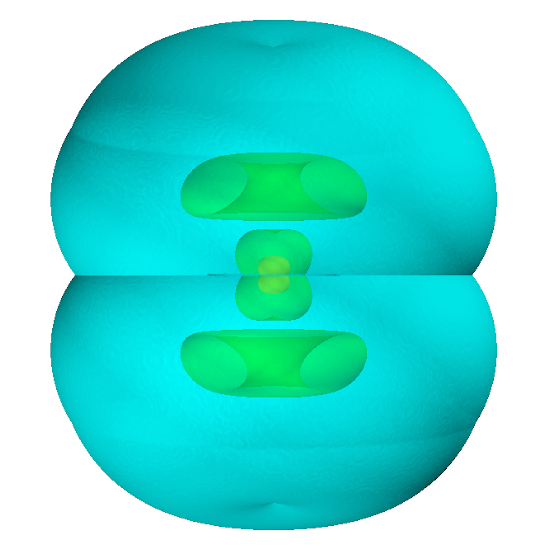
\includegraphics[width=1\linewidth]{electron-1} \\ а)
    \end{minipage}
    \hfill
    \begin{minipage}[b][][b]{0.49\linewidth}\centering
        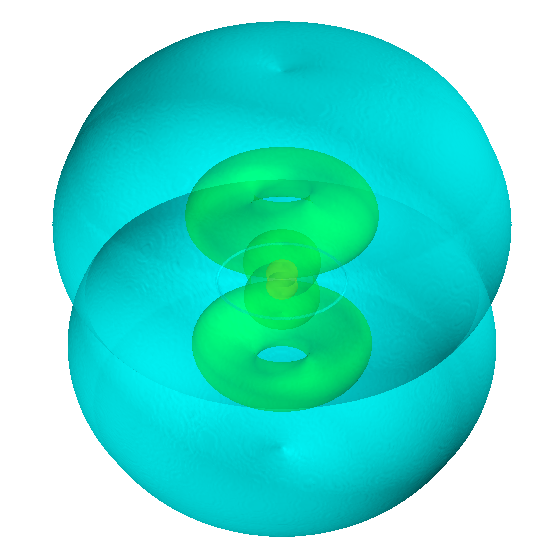
\includegraphics[width=1\linewidth]{electron-2} \\ б)
    \end{minipage}
    \caption{Электронная плотность, соответствующая <<отрицательному>> спину углерода в кластере Al4C6 в двух проекциях}
    \label{fig:electron-densities}
\end{figure}

\FloatBarrier
